\documentclass[12pt]{article}
\usepackage{amsmath, amssymb, amsthm}
\usepackage{graphicx}
\usepackage{booktabs}
\usepackage{float}
\usepackage[margin=1in]{geometry}
\usepackage{setspace}
\usepackage{natbib}
\usepackage[hidelinks]{hyperref}
\usepackage{listings}
\usepackage{xcolor}
\usepackage{caption}
\usepackage{subcaption}
\usepackage{enumitem}

\definecolor{codebg}{RGB}{248,248,248}
\lstset{
  basicstyle=\ttfamily\small,
  backgroundcolor=\color{codebg},
  frame=single,
  breaklines=true,
  showstringspaces=false,
}

% Safe figure helper: renders the figure if the file exists,
% otherwise prints a labelled placeholder so the document still compiles.
\newcommand{\safefig}[3]{%
  \IfFileExists{#1}{%
    \begin{figure}[H]
      \centering
      \includegraphics[width=0.92\textwidth]{#1}
      \caption{#2}
      \label{#3}
    \end{figure}
  }{%
    \begin{figure}[H]
      \centering
      \fbox{\parbox{0.92\textwidth}{\centering\textit{Figure not yet generated. Run the pipeline scripts to produce \texttt{\detokenize{#1}}.}}}
      \caption{#2 [placeholder]}
      \label{#3}
    \end{figure}
  }%
}

\begin{document}
\begin{titlepage}
    \centering
    \vspace*{3cm}
    {\Huge \textbf{Merton Jump-Diffusion: Pricing and Harvesting the Equity Jump Risk Premium} \par}
    \vspace{1.5cm}
    {\large Stochastic Processes --- Final Group Project \par}
    \vspace{2cm}
    {\Large Group 3 \par}
    \vspace{1cm}
    {\large May 5, 2026 \par}
    \vfill
\end{titlepage}

\section*{Literature Review}

The literature on asset price modelling has evolved considerably over the past five decades, moving well beyond the classical Black--Scholes framework in response to persistent empirical evidence that real financial markets are richer and more complex than any simple diffusion model can capture. This review traces that evolution across four connected areas. We begin with the foundational jump-diffusion models of Merton (1976) and Kou (2002), which introduced discontinuous price dynamics into option pricing theory, and the empirical diagnostics of Carr and Wu (2003), which confirmed that jumps are genuinely present in market data. We then turn to Eraker, Johannes, and Polson (2003), who demonstrated that both return jumps and volatility jumps are needed to fit index data, and discuss how self-exciting Hawkes processes extend this insight by allowing jump intensity to vary endogenously. Finally, we review the deep learning approach of Agram, \O{}ksendal, and Rems (2024), who address the hedging problem in incomplete jump-diffusion markets using neural network methods.

\subsection*{Classical Jump-Diffusion Processes}

The starting point for any study of discontinuous price dynamics is the Black--Scholes model, which assumes that the stock price follows a geometric Brownian motion with constant variance. While analytically tractable and elegant, the model has two well-known empirical failures. First, real return distributions exhibit leptokurtosis, with heavier tails than any normal distribution can accommodate. Second, implied volatilities extracted from observed option prices form a systematic skew or smile across strikes and maturities, rather than remaining flat as the model predicts. Both failures point in the same direction: actual price processes contain sudden, discontinuous moves that a continuous diffusion cannot generate.

Merton (1976) was the first to formally address this by adding a Poisson-driven jump process to geometric Brownian motion. He modelled the total change in the stock price as the sum of an ordinary diffusive component, representing the gradual arrival of information, and an abnormal component, representing the sudden impact of firm-specific news. Formally, the stock price dynamics are
\begin{equation}
\frac{dS}{S} = (\alpha - \lambda k)\,dt + \sigma\,dZ + dq,
\end{equation}
where $\alpha$ is the instantaneous expected return, $\sigma^2$ is the diffusive variance conditional on no jump, $dZ$ is a standard Brownian motion, $q(t)$ is an independent Poisson process with arrival rate $\lambda$, and $k \equiv E(Y-1)$ is the expected percentage price change per jump, with $Y$ denoting the random jump size multiplier. To price options under these dynamics, Merton observed that a riskless hedging portfolio cannot be constructed when jumps are present, since jump risk cannot be perfectly replicated by any portfolio of the stock and a risk-free bond. Under the special case where $Y$ is lognormally distributed, assuming that jump risk is non-systematic and therefore unpriced, this yields the Merton pricing formula
\begin{equation}
F(S,\tau) = \sum_{n=0}^{\infty} \frac{e^{-\lambda\tau}(\lambda\tau)^n}{n!}\,W\!\left(S X_n e^{-\lambda k\tau},\,\tau;\,E,\,\sigma^2,\,r\right),
\end{equation}
where $W(\cdot)$ is the standard Black--Scholes formula, $\tau$ is the time to expiration, $E$ is the exercise price, $r$ is the risk-free rate, and $X_n$ captures the cumulative jump factor conditional on $n$ jumps. Intuitively, the formula is an infinite weighted average of Black--Scholes prices, one for each possible number of jumps, with Poisson probabilities as weights, and reduces to Black--Scholes when $\lambda = 0$.

Despite its appeal, Merton's model has two notable limitations. Jump intensity $\lambda$ is constant, so the model cannot accommodate periods of elevated crash risk or jump clustering. Furthermore, normally distributed jump sizes imply symmetric tails, contradicting the well-documented finding that large negative equity returns are far more common than equally large positive returns.

Kou (2002) addressed both shortcomings by replacing the normal jump size distribution with an asymmetric double-exponential distribution. The asset price dynamics are
\begin{equation}
\frac{dS(t)}{S(t^-)} = \mu\,dt + \sigma\,dW(t) + d\!\left(\sum_{i=1}^{N(t)}(V_i - 1)\right),
\end{equation}
where $W(t)$ is a standard Brownian motion, $N(t)$ is a Poisson process with rate $\lambda$, and $\{V_i\}$ are i.i.d.\ non-negative random variables such that $Y = \log V$ has the density
\begin{equation}
f_Y(y) = p\cdot\eta_1 e^{-\eta_1 y}\mathbf{1}_{\{y\geq 0\}} + q\cdot\eta_2 e^{\eta_2 y}\mathbf{1}_{\{y < 0\}},\quad \eta_1 > 1,\; \eta_2 > 0,
\end{equation}
where $p$ and $q = 1-p$ are the probabilities of upward and downward jumps, and $1/\eta_1$ and $1/\eta_2$ are their respective mean sizes. The asymmetry between $\eta_1$ and $\eta_2$ directly captures the observation that market crashes are typically sharper than market rallies, which is particularly relevant for a technology-heavy index like the Nasdaq-100.

Beyond its empirical realism, the double-exponential distribution carries a significant mathematical advantage. Because exponential distributions are memoryless, the overshoot beyond a boundary also follows an exponential distribution and is conditionally independent of the first passage time. This structure enables closed-form solutions for path-dependent instruments --- barrier options, lookback options, and perpetual American options --- that are unavailable under Merton's normal jump specification. For European options, the pricing formula takes the form of a Poisson-weighted sum
\begin{equation}
f_n(S,\tau) = W\!\left(S,\,\tau;\,E,\,\sigma^2 + \frac{n\delta^2}{\tau},\,r\right),
\end{equation}
where $\delta^2$ is the variance of the logarithmic jump size and $f_n$ is the option price conditional on exactly $n$ jumps. Kou (2002) showed that the model reproduces the leptokurtic feature of daily returns and generates the asymmetric volatility skew observed in equity options, making it substantially more flexible than Merton's specification with a similarly parsimonious parameter set.

A limitation shared by both models is that jump intensity $\lambda$ is constant. Carr and Wu (2003) approached this problem from a different angle: rather than proposing a new parametric model, they asked whether one can determine directly from observed option prices, without committing to any specific model, whether the underlying process contains a continuous component, a jump component, or both. The key insight is that the short-maturity behaviour of out-of-the-money (OTM) options is a sensitive diagnostic of the underlying process. Under a purely continuous diffusion, OTM option prices decay at the exponentially fast rate $O(e^{-c/T})$ for some constant $c > 0$. Under any process with a jump component, a single jump can bring an OTM option into the money at any moment, so prices decay only at the much slower rate $O(T)$. Carr and Wu formalised this through a decomposition of the time value of a European option,
\begin{equation}
TV_0(K,T) = e^{-rT}\int_0^T\!\left[\tfrac{1}{2}q(K,t)K^2\,E_0\!\left[\sigma_t^2\,\big|\,F_{t^-}=K\right] + E_0\!\left[F_{t^-}\,v^0_t(k)\right]\right]dt,
\end{equation}
showing how the continuous martingale component and the jump compensator each contribute to option prices. They then proposed plotting $\ln(P/T)$ against $\ln T$ --- a term decay plot --- and reading off the slope at short maturities. A flat slope near zero for OTM options signals a jump component; a sharply negative slope signals a pure diffusion; intermediate ATM slopes distinguish finite-variation from infinite-variation jump processes.

Applying this methodology to S\&P 500 index options from April 1999 to May 2000, Carr and Wu found strong evidence for both a continuous and a jump component in index dynamics. The continuous component was persistently present throughout the sample, while the jump component varied substantially over time and was negatively correlated (around $-0.58$) with the level of implied volatility. This finding validates the general approach of Merton and Kou while simultaneously pointing to their most important limitation: they cannot accommodate the time-varying nature of jump intensity. For any empirical project working with index options, the Carr--Wu diagnostic therefore provides a model-free first check before any parametric calibration is attempted.

\subsection*{Stochastic Volatility and Jump Clustering}

While Merton and Kou represent genuine progress over Black--Scholes, both assume constant jump intensity, an assumption the evidence increasingly challenged. A natural baseline for richer dynamics is the stochastic volatility (SV) model of Heston (1993), in which the instantaneous variance $V_t$ follows a mean-reverting square-root process. Even this model falls short, as Eraker, Johannes, and Polson (2003) demonstrated through a careful likelihood-based study of S\&P 500 and Nasdaq 100 daily returns. The pure SV model still fails to generate the extreme returns observed during crises without implausibly large diffusive shocks; on the day of the October 1987 crash, it would require a return innovation of nearly eight standard deviations to produce the observed $-23\%$ move.

The natural fix is to add return jumps, giving the SVJ model. In this specification the log-price $Y_t = \log S_t$ satisfies
\begin{equation}
dY_t = \mu\,dt + \sqrt{V_{t^-}}\,dW^Y_t + \xi^Y\,dN^Y_t,
\end{equation}
where $N^Y_t$ is a Poisson process with constant intensity $\lambda^Y$ and $\xi^Y \sim N(\mu_Y, \sigma_Y^2)$ is the normally distributed jump size. The variance process evolves as
\begin{equation}
dV_t = \kappa(\theta - V_t)\,dt + \sigma_v\sqrt{V_t}\,dW^V_t,
\end{equation}
with $\mathrm{Corr}(dW^Y_t, dW^V_t) = \rho\,dt$ capturing the leverage effect. Adding return jumps reduces the estimated diffusive volatility of volatility $\sigma_v$ and the speed of mean reversion $\kappa$, and jumps account for roughly 15\% of total return variance in the SVJ model.

However, the SVJ model is itself misspecified in a revealing way. Under a constant-intensity Poisson assumption averaging roughly 1.5 arrivals per year, the SVJ algorithm identifies three separate jump arrivals during the week of the 1987 crash alone --- an implausible outcome under the model's own distributional assumptions. This clustering signals a systematic misfit: the model has no mechanism to link the occurrence of one jump to the likelihood of the next.

The solution proposed by Eraker et al.\ is to allow volatility itself to jump. In the SVCJ model --- stochastic volatility with contemporaneous jumps --- the variance equation becomes
\begin{equation}
dV_t = \kappa(\theta - V_t)\,dt + \sigma_v\sqrt{V_{t^-}}\,dW^V_t + \xi^V\,dN_t,
\end{equation}
where $N_t$ is shared with the return-jump process, $\xi^V \sim \mathrm{Exp}(\mu_V)$ ensures positive volatility jumps, and the return jump conditional on the volatility jump is $\xi^Y \mid \xi^V \sim N(\mu_Y + \rho_J\xi^V, \sigma_Y^2)$. A volatility jump provides a persistent shock to the conditional distribution of future returns, whereas a return jump is transient: it shifts today's price but leaves tomorrow's variance unaffected. In the SVCJ model, the 1987 crash week is explained by a single large contemporaneous jump driving a $-14\%$ return while simultaneously pushing annualised volatility from around 40\% to just over 50\%, after which volatility mean-reverts gradually --- a far more economically coherent story than three independent Poisson arrivals in a single week.

Estimation is carried out by Markov Chain Monte Carlo (MCMC), which recovers the full joint posterior of parameters and latent states --- spot volatility, jump times, and jump sizes --- simultaneously. Formal Bayes factors strongly favour the SVCJ specification: the log Bayes factor comparing the SV model to the SVIJ specification (independent jumps in returns and volatility) is 59.45, constituting decisive evidence in favour of the richer model by the Kass--Raftery scale. From an option-pricing perspective, volatility jumps steepen the implied volatility smile and generate the characteristic ``hook'' for in-the-money options, a feature entirely absent from the SVJ model.

Despite these improvements, the SVCJ model still assumes constant jump intensities $\lambda^Y$ and $\lambda^V$, and the authors' own diagnostics undermine this assumption: jump times cluster in crisis periods, inconsistent with a homogeneous Poisson process. Hawkes (1971) self-exciting processes provide the natural mechanism for endogenising this behaviour. In a Hawkes process, the intensity $\lambda(t)$ increases each time a jump arrives and then decays back toward a baseline level:
\begin{equation}
\lambda(t) = \mu + \int_{-\infty}^{t}\varphi(t-s)\,dN(s),
\end{equation}
where $\mu > 0$ is the background intensity and $\varphi(\cdot) \geq 0$ is the excitation kernel, typically taken to be $\varphi(u) = \alpha e^{-\beta u}$ with $\alpha < \beta$ to ensure stationarity. Each jump raises $\lambda(t)$ by $\alpha$, making the next arrival more likely; but this excess intensity decays at rate $\beta$, so the process eventually returns to $\mu$. This structure captures both the clustering of jumps during market stress and their eventual dissipation.

Gonzato and Sgarra (2021) provide a recent example of how self-exciting jumps can be used in a financial jump model. They study a specification in which the arrival of one jump increases the probability of future jumps, allowing the model to reproduce clustering during turbulent periods. Although their empirical application is to the oil market, the mechanism is directly relevant for equity index options: crashes and earnings-related shocks are rarely isolated events, and a constant Poisson intensity may underestimate the persistence of jump risk after the first shock.

Calibration typically proceeds by maximum likelihood for moderate sample sizes or Sequential Monte Carlo (SMC) when jump sizes are also stochastic and the state space becomes high-dimensional. For the present project, the Hawkes framework serves primarily as a conceptual benchmark: the Merton and Kou models, with their constant $\lambda$, sit at one extreme of the spectrum, while the Hawkes model, with fully endogenous intensity, sits at the other.

\subsection*{Machine Learning Extensions of Stochastic Processes}

Both classical jump-diffusion models and richer stochastic volatility plus jump specifications produce analytical solutions only in special cases. Once one moves to genuinely incomplete markets --- where the number of independent risk sources exceeds the number of traded assets, which is the generic situation when multiple Brownian motions or Poisson processes are present --- closed-form hedging strategies cease to exist. This is precisely the setting studied by Agram, \O{}ksendal, and Rems (2024), who propose a deep learning approach to the minimal variance (quadratic) hedging problem.

The market model considered is a single risky asset whose price $S(t)$ satisfies
\begin{equation}
dS(t) = S(t^-)\!\left[\alpha(t)\,dt + \sigma(t)\,dB(t) + \int_{\mathbb{R}^*}\!\gamma(t,\zeta)\,\tilde{N}(dt,d\zeta)\right],\quad S(0)>0,
\end{equation}
where $B(t)$ is an $m$-dimensional Brownian motion, $\tilde{N}$ is a $k$-dimensional compensated Poisson random measure, and $\alpha, \sigma, \gamma$ are deterministic and bounded. The market is incomplete when $m > 1$ or $k > 1$. For a self-financing portfolio $\pi(t)$ representing the fraction of wealth invested in the risky asset, the wealth process $X(t)$ evolves accordingly, and the hedging objective is to minimise
\begin{equation}
J(z,\pi) = E\!\left[\tfrac{1}{2}\bigl(X^{z,\pi}(T) - F\bigr)^2\right].
\end{equation}
Agram et al.\ frame this as a Stackelberg game: the first player chooses the initial endowment $z$ (the option price), and the second then selects the optimal portfolio $\hat{\pi}$ given that endowment. The main theoretical result is that the minimal variance price can be written as an expectation under a specific equivalent martingale measure $Q^*$:
\begin{equation}
\hat{z} = E^{Q^*}[F],
\end{equation}
where $Q^*$ is characterised by a Radon--Nikod\'{y}m derivative involving $G(t) = -\alpha(t)/\bigl(\sigma^2(t) + \int\gamma^2(t,\zeta)\,\nu(d\zeta)\bigr)$. Crucially, $Q^*$ is a genuine positive equivalent martingale measure rather than a signed measure, which is not guaranteed in general incomplete markets.

In more complex settings, the price integral $E^{Q^*}[F]$ and the corresponding portfolio must be computed numerically. Agram et al.\ propose a neural network algorithm combining a feed-forward layer to estimate the option price $z_0$ with a two-layer Long Short-Term Memory (LSTM) network to approximate the optimal portfolio $\pi_t$ at each time step. The LSTM architecture is well suited to this problem: the optimal portfolio is adapted to the filtration generated by the price process, so past observations are relevant for each decision, and LSTM cells maintain a memory state that allows the network to learn how past jumps affect the current hedging ratio --- especially valuable when latent volatility evolves stochastically.

The algorithm is tested on four model environments. In the Black--Scholes benchmark, it converges to the theoretical option price of 0.500 and recovers the delta hedge accurately. For the Merton jump-diffusion model, the minimal variance price is $\hat{z} = 0.519$, exceeding the Merton model's own price of 0.515. This difference arises because the Merton approach assumes jump risk is diversifiable and therefore receives no risk premium, whereas the minimal variance approach explicitly prices the unhedgeable component. The practical consequence is stark: standard Merton delta hedging produces a skewed distribution of hedging errors --- small gains most of the time but occasional large losses when a jump occurs --- whereas the minimal variance hedge yields a roughly symmetric error distribution with virtually no extreme losses. The algorithm also converges to a reasonable estimate for the Kou double-exponential model, where no closed-form equivalent martingale measure price exists.

The main limitations concern scalability and interpretability: convergence slows after a few thousand training epochs, training time grows substantially with the number of time-discretisation steps, and accuracy decreases as option maturity lengthens due to accumulating discretisation errors. Despite these drawbacks, the framework represents a genuine advance over purely analytical methods because it handles models --- such as the Kou model with two-sided jumps, or future extensions incorporating stochastic volatility and self-exciting jump intensity --- where closed-form solutions simply do not exist.

\subsection*{Research Frontier and Connection to Our Project}

Taken together, the literature reviewed above traces a coherent arc from the first principled treatment of jump risk through to the modern machine learning frontier. Merton (1976) broke with the continuity assumption of Black--Scholes and provided the first tractable framework for option pricing under jump risk. Kou (2002) extended this by replacing the symmetric normal jump distribution with an asymmetric double-exponential, capturing the empirical reality that crashes are sharper than rallies and enabling closed-form solutions for a wider class of options. Carr and Wu (2003) confirmed empirically that both continuous and jump components are present in S\&P 500 index options, and that their relative importance varies systematically over time. Eraker, Johannes, and Polson (2003) demonstrated through Bayesian estimation that stochastic volatility alone is insufficient and that both return and volatility jumps are necessary to fit index data. The Hawkes framework provides one natural way to endogenise jump clustering, while the deep learning approach of Agram et al.\ (2024) addresses the pricing and hedging problem in incomplete markets where analytical solutions are unavailable.

Several unresolved tensions emerge from this literature. The most fundamental is the trade-off between empirical richness and analytical tractability. The Merton and Kou models are estimable but too restrictive, unable to accommodate time-varying jump intensity or persistent volatility jumps. The SVCJ model fits the data better but requires computationally intensive MCMC estimation. The Hawkes framework adds endogenous clustering but raises its own estimation challenges and has not been as thoroughly tested against option-implied data as the parametric jump-diffusion models. The deep learning approach of Agram et al.\ is the most flexible but sacrifices interpretability.

A second tension concerns the identification of jump risk premia. Both Merton and Kou price options without explicitly modelling the compensation that investors require for bearing jump risk. The finding that the minimal variance price exceeds the Merton price aligns with the expectation that implied volatilities should be systematically above the levels implied by the physical measure. For a technology index like the Nasdaq-100, where sector-specific crashes can be swift and severe, this premium is likely to be economically significant and is one of the central quantities of interest in the present project.

A third consideration is the diagnostic value of the Carr--Wu term decay methodology. Before committing to any parametric model, plotting term decay curves for short-maturity options will indicate whether a finite-variation jump component of the Merton or Kou type is sufficient, or whether the data hints at infinite-variation or time-varying intensity dynamics. A flat OTM slope near zero at short maturities would confirm a Poisson-type jump component, while a clearly negative slope would point toward infinite-variation L\'{e}vy components or stochastic volatility extensions.

Looking forward, the literature suggests several natural extensions. One is to replace the constant Poisson intensity in the Merton and Kou models with a Hawkes self-exciting intensity, capturing jump clustering during stress periods without the full computational burden of MCMC. Another is to apply the LSTM-based hedging algorithm of Agram et al.\ to produce out-of-sample hedging strategies for QQQ options that are more robust to jump risk than standard delta hedging. A third is to estimate the models jointly from time-series returns and option prices to obtain internally consistent estimates of both the physical and risk-neutral jump parameters. Each extension would move the analysis closer to the frontier of what the recent literature has demonstrated is both theoretically justified and empirically important.

\paragraph{Literature Review Summary.}
The literature reviewed in this chapter documents a clear progression in the understanding and modelling of discontinuous price dynamics. Black--Scholes fails on two empirically important counts: it cannot generate the heavy tails and negative skewness of real return distributions, and it produces a flat implied volatility surface rather than the skew or smile that options markets consistently display. Merton (1976) introduced a Poisson-driven jump process alongside the diffusion and derived an option pricing formula that nests Black--Scholes as a special case, but relies on symmetric normal jump sizes and a constant arrival rate. Kou (2002) improved on the first assumption by replacing the normal distribution with an asymmetric double-exponential, while both models leave jump intensity constant. Carr and Wu (2003) confirmed empirically that jumps are present in index options data and that their importance varies over time. Eraker, Johannes, and Polson (2003) showed through Bayesian estimation that stochastic volatility alone is insufficient, and that contemporaneous jumps in both returns and volatility are decisively preferred by the data. Hawkes processes extend this insight by formalising the endogenous clustering of jumps during market stress. Finally, the deep learning framework of Agram et al.\ (2024) provides a formal confirmation that jump risk commands a positive premium in incomplete markets, and that ignoring it leads to systematically biased hedges and unexpected losses.

No single model explains financial markets perfectly: each involves a compromise between empirical fit, analytical tractability, and estimation feasibility. This honest recognition of limitations is precisely what motivates continued research into stochastic jump-diffusion processes and makes the study of jump risk premia in real option markets --- the focus of the present project --- both timely and relevant.

\newpage
\section*{Mathematical Derivations}
\label{sec:mathematical_derivations}

This section fixes the mathematical notation used in the pricing, Monte Carlo, COS, calibration, and hedging parts of the project. We focus on the Merton jump-diffusion model as the main model and on the Kou double-exponential jump model as the benchmark extension. The goal is not only to state the formulas, but to show why the drift correction, characteristic functions, and incompleteness results arise naturally.

\subsection*{Physical and Risk-Neutral Dynamics}

Let $(\Omega,\mathcal{F},(\mathcal{F}_t)_{t\geq 0},\mathbb{P})$ be a filtered probability space supporting a Brownian motion $W_t^{\mathbb{P}}$ and a Poisson process $N_t^{\mathbb{P}}$ with intensity $\lambda^{\mathbb{P}}$. The jump sizes are represented by i.i.d. random variables $J_i$, independent of both $W^{\mathbb{P}}$ and $N^{\mathbb{P}}$. If $Y_i=e^{J_i}$ denotes the gross jump multiplier, then a jump changes the stock price from $S_{t^-}$ to $S_t=S_{t^-}Y_i$.

Under the physical measure $\mathbb{P}$, the model can be written as
\begin{equation}
\frac{dS_t}{S_{t^-}}
= \left(\mu - \lambda^{\mathbb{P}}\kappa^{\mathbb{P}}\right)dt
+ \sigma dW_t^{\mathbb{P}}
+ (e^{J}-1)dN_t^{\mathbb{P}},
\label{eq:p_dynamics}
\end{equation}
where
\begin{equation}
\kappa^{\mathbb{P}} = \mathbb{E}^{\mathbb{P}}[e^J-1]
\label{eq:kappa_p}
\end{equation}
is the expected percentage jump size under $\mathbb{P}$. The physical parameters describe the historical behaviour of returns and will later be estimated from high-frequency QQQ data and jump detection tests.

For pricing, we work under a risk-neutral measure $\mathbb{Q}$. The discounted stock price must be a martingale under $\mathbb{Q}$, so the drift is replaced by the risk-free rate and corrected for the expected jump contribution. The risk-neutral dynamics are
\begin{equation}
\frac{dS_t}{S_{t^-}}
= \left(r - \lambda^{\mathbb{Q}}\kappa^{\mathbb{Q}}\right)dt
+ \sigma dW_t^{\mathbb{Q}}
+ (e^{J}-1)dN_t^{\mathbb{Q}},
\label{eq:q_dynamics_general}
\end{equation}
where
\begin{equation}
\kappa^{\mathbb{Q}} = \mathbb{E}^{\mathbb{Q}}[e^J-1].
\label{eq:kappa_q}
\end{equation}
In the rest of this section we suppress the superscript $\mathbb{Q}$ and write $\lambda$ and $\kappa$ for risk-neutral quantities. The difference between the physical jump intensity $\lambda^{\mathbb{P}}$ and the calibrated risk-neutral intensity $\lambda^{\mathbb{Q}}$ is economically important: it is one way to measure the jump risk premium.

\subsection*{Change of Measure and Girsanov Argument}

Before deriving the Merton stock-price dynamics, we briefly clarify how the passage from the physical measure $\mathbb{P}$ to the pricing measure $\mathbb{Q}$ is represented in our notation. The passage from $\mathbb{P}$ to $\mathbb{Q}$ can be viewed as a change of measure. For the Brownian part, Girsanov's theorem changes only the drift. In the simple constant-coefficient case, define
\begin{equation}
\frac{d\mathbb{Q}}{d\mathbb{P}}\bigg|_{\mathcal{F}_T}
=\exp\left(-\theta W_T^{\mathbb{P}}-\frac{1}{2}\theta^2T\right),
\qquad
W_t^{\mathbb{Q}}=W_t^{\mathbb{P}}+\theta t.
\label{eq:girsanov_density}
\end{equation}
Then $W_t^{\mathbb{Q}}$ is a Brownian motion under $\mathbb{Q}$, and the Brownian drift can be adjusted so that the discounted stock price is a martingale. In a pure diffusion model this would pin down the unique risk-neutral measure. In a jump-diffusion model, however, the jump intensity and jump-size distribution may also change under the pricing measure. Since jump risk is not perfectly hedgeable, no-arbitrage does not determine this jump-risk adjustment uniquely. For this reason, our empirical implementation estimates physical jump parameters from returns but calibrates risk-neutral jump parameters directly from option prices. This is the practical link between Girsanov's theorem, market incompleteness, and the jump risk premium discussed in this project \citep{Shreve2004}.

\subsection*{From the Log-Price to the Stock-Price SDE}

Define the log-price process
\begin{equation}
X_t=\log S_t.
\label{eq:log_price}
\end{equation}
For a finite-activity jump-diffusion, the risk-neutral log-price dynamics are
\begin{equation}
dX_t=
\left(r-\lambda\kappa-\frac{1}{2}\sigma^2\right)dt
+\sigma dW_t^{\mathbb{Q}}+JdN_t.
\label{eq:log_sde}
\end{equation}
The term $-\frac{1}{2}\sigma^2$ is the usual It\^{o} correction from geometric Brownian motion, while $-\lambda\kappa$ compensates for the average jump growth.

To recover the stock-price dynamics, apply It\^{o}'s formula for jump processes to $S_t=e^{X_t}$. Between jumps, the continuous part gives
\begin{equation}
\frac{dS_t}{S_t}=
\left(r-\lambda\kappa\right)dt+\sigma dW_t^{\mathbb{Q}}.
\end{equation}
At a jump time, $\Delta X_t=J$, hence
\begin{equation}
\Delta S_t=S_{t^-}(e^J-1).
\end{equation}
Combining the continuous and jump parts gives exactly
\begin{equation}
\frac{dS_t}{S_{t^-}}=
(r-\lambda\kappa)dt+\sigma dW_t^{\mathbb{Q}}+(e^J-1)dN_t,
\label{eq:merton_sde_final}
\end{equation}
which is the Merton jump-diffusion SDE used throughout the project.

\subsection*{Martingale Condition}

The risk-neutral drift in Equation~\eqref{eq:merton_sde_final} is chosen so that the discounted price $e^{-rt}S_t$ is a $\mathbb{Q}$-martingale. Let $\tau=T-t$. Solving Equation~\eqref{eq:log_sde} over $[t,T]$ gives
\begin{equation}
S_T=S_t\exp\left[
\left(r-\lambda\kappa-\frac{1}{2}\sigma^2\right)\tau
+\sigma(W_T^{\mathbb{Q}}-W_t^{\mathbb{Q}})
+\sum_{i=1}^{N_\tau}J_i
\right].
\label{eq:st_solution}
\end{equation}
Since the Brownian and jump parts are independent,
\begin{align}
\mathbb{E}_t^{\mathbb{Q}}[S_T]
&=S_t e^{(r-\lambda\kappa-\frac12\sigma^2)\tau}
\mathbb{E}^{\mathbb{Q}}\!\left[e^{\sigma(W_T-W_t)}\right]
\mathbb{E}^{\mathbb{Q}}\!\left[e^{\sum_{i=1}^{N_\tau}J_i}\right].
\end{align}
The Brownian expectation is
\begin{equation}
\mathbb{E}^{\mathbb{Q}}\!\left[e^{\sigma(W_T-W_t)}\right]
=e^{\frac12\sigma^2\tau},
\end{equation}
and the compound Poisson expectation is
\begin{equation}
\mathbb{E}^{\mathbb{Q}}\!\left[e^{\sum_{i=1}^{N_\tau}J_i}\right]
=\exp\left(\lambda\tau\bigl(\mathbb{E}^{\mathbb{Q}}[e^J]-1\bigr)\right)
=e^{\lambda\kappa\tau}.
\end{equation}
Therefore,
\begin{equation}
\mathbb{E}_t^{\mathbb{Q}}[S_T]=S_t e^{r\tau},
\end{equation}
and hence
\begin{equation}
\mathbb{E}_t^{\mathbb{Q}}\left[e^{-r(T-t)}S_T\right]=S_t.
\label{eq:martingale_result}
\end{equation}
Thus the discounted stock price is a martingale under $\mathbb{Q}$, which is the no-arbitrage condition needed for risk-neutral valuation.

\subsection*{Characteristic Function of the Merton Model}

Fourier and COS pricing methods require the characteristic function of $X_T=\log S_T$. From Equation~\eqref{eq:st_solution}, for any real $u$,
\begin{equation}
\begin{aligned}
\phi_X(u;t,T)
&= \mathbb{E}_t^{\mathbb{Q}}\!\left[e^{iuX_T}\right] \\
&= \exp\!\Bigg(
iu\Big[x_t+\Big(r-\lambda\kappa-\tfrac12\sigma^2\Big)\tau\Big]
-\tfrac12\sigma^2u^2\tau \\
&\qquad\qquad
+\lambda\tau\big(\Psi_J(u)-1\big)
\Bigg).
\end{aligned}
\label{eq:general_cf}
\end{equation}
where
\begin{equation}
\Psi_J(u)=\mathbb{E}^{\mathbb{Q}}[e^{iuJ}]
\label{eq:jump_cf}
\end{equation}
is the characteristic function of the log-jump size.

In the Merton model,
\begin{equation}
J\sim N(\mu_J,\sigma_J^2).
\end{equation}
Therefore,
\begin{equation}
\Psi_J(u)=\exp\left(iu\mu_J-\frac12u^2\sigma_J^2\right),
\label{eq:merton_jump_cf}
\end{equation}
and
\begin{equation}
\kappa=\mathbb{E}[e^J-1]
=\exp\left(\mu_J+\frac12\sigma_J^2\right)-1.
\label{eq:merton_kappa}
\end{equation}
Substituting Equations~\eqref{eq:merton_jump_cf} and~\eqref{eq:merton_kappa} into Equation~\eqref{eq:general_cf} gives the Merton characteristic function used in our COS engine.

\subsection*{Merton Pricing Formula}

For a European call option with payoff $(S_T-K)^+$, the risk-neutral price is
\begin{equation}
C(t,S_t)=e^{-r\tau}\mathbb{E}_t^{\mathbb{Q}}[(S_T-K)^+].
\label{eq:risk_neutral_call}
\end{equation}
The key step is to condition on the number of jumps. Since $N_\tau\sim \mathrm{Poisson}(\lambda\tau)$,
\begin{equation}
C(t,S_t)=\sum_{n=0}^{\infty}\mathbb{P}(N_\tau=n)\,
 e^{-r\tau}\mathbb{E}_t^{\mathbb{Q}}[(S_T-K)^+\mid N_\tau=n].
\label{eq:condition_on_n}
\end{equation}
Conditional on $N_\tau=n$, the sum of log-jumps is normal:
\begin{equation}
\sum_{i=1}^{n}J_i\sim N(n\mu_J,n\sigma_J^2).
\end{equation}
Thus, conditional on $n$ jumps, the terminal log-price is still normally distributed. It can be represented as a Black--Scholes log-price with adjusted volatility
\begin{equation}
\sigma_n^2=\sigma^2+\frac{n\sigma_J^2}{\tau},
\label{eq:sigma_n}
\end{equation}
and adjusted drift parameter
\begin{equation}
r_n=r-\lambda\kappa+\frac{n\mu_J}{\tau}+\frac{n\sigma_J^2}{2\tau}.
\label{eq:r_n}
\end{equation}
The conditional Black--Scholes representation is discounted at $r_n$, while the original risk-neutral payoff in Equation~\eqref{eq:risk_neutral_call} is discounted at $r$. Therefore the conditional price contributes an additional factor $e^{(r_n-r)\tau}$. Using Equation~\eqref{eq:r_n},
\begin{equation}
e^{(r_n-r)\tau}
=\exp\left(-\lambda\kappa\tau+n\mu_J+\frac12n\sigma_J^2\right)
=e^{-\lambda\kappa\tau}(1+\kappa)^n,
\label{eq:rn_adjustment}
\end{equation}
because $1+\kappa=\exp(\mu_J+\frac12\sigma_J^2)$. Hence
\begin{equation}
e^{-\lambda\tau}\frac{(\lambda\tau)^n}{n!}e^{(r_n-r)\tau}
=
e^{-\lambda(1+\kappa)\tau}
\frac{(\lambda(1+\kappa)\tau)^n}{n!}.
\label{eq:lambda_prime_derivation}
\end{equation}
Defining $\lambda'=\lambda(1+\kappa)$, the Merton price becomes
\begin{equation}
C^{\mathrm{Merton}}(S,K,\tau)
=\sum_{n=0}^{\infty}
e^{-\lambda'\tau}\frac{(\lambda'\tau)^n}{n!}
C^{\mathrm{BS}}(S,K,\tau,r_n,\sigma_n),
\label{eq:merton_price_formula}
\end{equation}
where
\begin{equation}
\lambda'=\lambda(1+\kappa)=\lambda\exp\left(\mu_J+\frac12\sigma_J^2\right).
\label{eq:lambda_prime}
\end{equation}
This formula is useful twice in our project. First, it provides a fast semi-closed-form benchmark for European option prices. Second, it will be used as a control variate and validation target for the Monte Carlo and COS implementations.

\subsection*{Market Incompleteness}

The Merton model is incomplete because jump risk cannot be perfectly replicated by continuously trading only the stock and the risk-free asset. The reason is simple but important.

Suppose an option has value $C(t,S_t)$. If the stock jumps from $S_{t^-}$ to $S_{t^-}e^J$, then the option value jumps by
\begin{equation}
\Delta C_t=C(t,S_{t^-}e^J)-C(t,S_{t^-}).
\label{eq:option_jump}
\end{equation}
A stock hedge holding $\Delta_t$ shares changes by
\begin{equation}
\Delta_t\Delta S_t=\Delta_t S_{t^-}(e^J-1).
\label{eq:stock_jump_hedge}
\end{equation}
For perfect replication at the jump time, we would need
\begin{equation}
C(t,S_{t^-}e^J)-C(t,S_{t^-})
=\Delta_tS_{t^-}(e^J-1)
\quad\text{for every possible }J.
\label{eq:jump_replication_condition}
\end{equation}
The right-hand side is linear in the jump multiplier $e^J$, while the option value is nonlinear in $S$. Except for a linear payoff, no single value of $\Delta_t$ can make Equation~\eqref{eq:jump_replication_condition} true for all possible jump sizes. Therefore the jump component creates unhedgeable risk.

This has two consequences. First, unlike the Black--Scholes model, no-arbitrage alone does not determine a unique equivalent martingale measure. Second, delta hedging leaves jump-related hedging error, motivating the minimum-variance hedge and tail-risk analysis used later in the project. This is consistent with the standard link between market completeness, replication, and uniqueness of the risk-neutral measure discussed in continuous-time asset pricing theory \citep{Shreve2004}.

\subsection*{Kou Double-Exponential Jump Model}

The Kou model keeps the same jump-diffusion structure but changes the distribution of the log-jump size. Instead of normal jumps, Kou assumes the asymmetric double-exponential density
\begin{equation}
f_J(j)=p\eta_1e^{-\eta_1 j}\mathbf{1}_{\{j\geq 0\}}
+q\eta_2e^{\eta_2 j}\mathbf{1}_{\{j<0\}},
\quad p+q=1,
\label{eq:kou_density}
\end{equation}
where $p$ is the probability of an upward jump and $q$ is the probability of a downward jump. The parameters $\eta_1$ and $\eta_2$ control the right and left tails. This asymmetry is useful for equity indices because downside jumps are usually sharper than upside jumps.

The characteristic function of the Kou jump size is
\begin{equation}
\Psi_J^{\mathrm{Kou}}(u)
=\frac{p\eta_1}{\eta_1-iu}
+\frac{q\eta_2}{\eta_2+iu}.
\label{eq:kou_jump_cf}
\end{equation}
The compensator is
\begin{equation}
\kappa_{\mathrm{Kou}}
=\mathbb{E}[e^J-1]
=\frac{p\eta_1}{\eta_1-1}
+\frac{q\eta_2}{\eta_2+1}-1,
\quad \eta_1>1.
\label{eq:kou_kappa}
\end{equation}
Therefore the Kou log-price characteristic function is obtained by substituting Equations~\eqref{eq:kou_jump_cf} and~\eqref{eq:kou_kappa} into the general formula~\eqref{eq:general_cf}. This makes Kou directly compatible with the same Fourier/COS framework as Merton.

The practical difference is that Merton uses normally distributed log-jumps, while Kou uses asymmetric exponential tails. Merton is simpler and gives a convenient Poisson-weighted Black--Scholes formula. Kou is better suited for modelling sharp downside moves and has special tractability for barrier and lookback options because the exponential distribution is memoryless.

\subsection*{Parameter Interpretation}

The parameters used in our Merton calibration have the following interpretation:
\begin{center}
\begin{tabular}{|c|p{6.5cm}|p{4.2cm}|}
\hline
Parameter & Financial meaning & Main effect on option surface \\
\hline
$\sigma$ & Continuous diffusive volatility & Controls the general level of implied volatility \\
\hline
$\lambda$ & Risk-neutral jump arrival intensity & Controls how much tail risk is priced \\
\hline
$\mu_J$ & Mean log-jump size & Controls the direction of skew; negative values generate downside skew \\
\hline
$\sigma_J$ & Standard deviation of log-jump size & Controls jump-size uncertainty and tail thickness \\
\hline
$\kappa$ & Expected percentage jump size, $\mathbb{E}[e^J-1]$ & Drift correction required for the martingale condition \\
\hline
\end{tabular}
\end{center}

This completes the theoretical input required by the later workstreams: the Monte Carlo engine uses the exact log-price representation, the COS engine uses the characteristic functions, the calibration step estimates the risk-neutral parameters from implied volatilities, and the hedging section uses incompleteness to motivate jump-aware hedging.

\newpage
\section*{Monte Carlo Pricing and Validation}
\label{sec:monte_carlo}

This section describes the Monte Carlo engine used to price European options under the Merton jump-diffusion model, following standard Monte Carlo principles used in financial engineering \citep{Glasserman2004}. The implementation is designed to be consistent with the risk-neutral dynamics derived in Section~\ref{sec:mathematical_derivations}, and the analytic Merton price in Equation~\eqref{eq:merton_price_formula} is used as the validation benchmark. The goal of this workstream is not only to simulate prices, but also to test convergence, compare variance-reduction methods, and generate reproducible numerical outputs for later calibration and hedging sections.

\subsection*{Risk-Neutral Simulation Scheme}

Under the risk-neutral Merton model, the log-price satisfies
\begin{equation}
X_T = X_0 + \left(r-\lambda\kappa-\frac12\sigma^2\right)T
+\sigma W_T + \sum_{i=1}^{N_T}J_i,
\label{eq:w3_terminal_logprice}
\end{equation}
where $N_T\sim \mathrm{Poisson}(\lambda T)$ and $J_i\sim N(\mu_J,\sigma_J^2)$. In the Monte Carlo code, the original jump intensity $\lambda$ is used for path simulation. The transformed intensity $\lambda'=\lambda(1+\kappa)$ appears only in the analytic Poisson-weighted Black--Scholes formula after the algebraic rearrangement shown in Equation~\eqref{eq:lambda_prime_derivation}. This distinction is important because the simulation follows the actual jump-count process, while the analytic formula rewrites the conditional pricing mixture.

For a European call option, each simulated terminal price produces the discounted payoff
\begin{equation}
\widehat{C}_m=e^{-rT}(S_T^{(m)}-K)^+,
\end{equation}
and the plain Monte Carlo estimator is
\begin{equation}
\widehat{C}_{MC}=\frac1M\sum_{m=1}^{M}\widehat{C}_m,
\qquad
\widehat{SE}=\frac{s(\widehat{C}_1,\ldots,\widehat{C}_M)}{\sqrt{M}},
\label{eq:w3_plain_mc}
\end{equation}
where $M$ is the number of simulated paths and $s(\cdot)$ is the sample standard deviation of discounted payoffs.

The implementation supports two equivalent simulation modes. For European payoffs, the terminal representation in Equation~\eqref{eq:w3_terminal_logprice} can be sampled directly in one step. For diagnostic purposes, the code also supports a time-grid version that simulates Brownian increments and Poisson jump arrivals over $N$ time steps. Since the log-price increments are sampled exactly over each interval, the time-grid experiment should be interpreted as a numerical stability check rather than as an Euler discretisation convergence study.

\subsection*{Variance Reduction Methods}

Three variance-reduction methods are implemented and compared against the plain Monte Carlo estimator. First, antithetic variates are used for the Brownian component. For each standard normal shock $Z$, the simulation also constructs a paired path using $-Z$. The jump component is drawn independently across the two paired branches. This keeps the negative correlation generated by the diffusion part, while avoiding an artificial coupling of jump arrivals across the antithetic pair.

Second, moment matching rescales the simulated terminal prices so that their sample mean matches the martingale target $S_0e^{rT}$ implied by Equation~\eqref{eq:martingale_result}. This finite-sample correction enforces the no-arbitrage mean condition on each simulation batch and reduces bias in the estimated terminal distribution, although it does not necessarily reduce the variance of the payoff estimator.

Third, a Black--Scholes control variate is used. Let $Y$ be the discounted Merton payoff and let $X$ be the discounted Black--Scholes payoff generated from the same Brownian shocks but with jumps removed. Since the exact Black--Scholes price $C^{BS}$ is known, the control-variate estimator is
\begin{equation}
\widehat{C}_{CV}=\overline{Y}-\widehat{\beta}(\overline{X}-C^{BS}),
\qquad
\widehat{\beta}=\frac{\widehat{\mathrm{Cov}}(Y,X)}{\widehat{\mathrm{Var}}(X)}.
\label{eq:w3_control_variate}
\end{equation}
Using the same Brownian shocks is essential: it creates a strong correlation between the Merton payoff and the control payoff, which is what makes the control variate effective. The jump component remains unhedged in the control, so the method reduces variance but does not remove jump risk.

\subsection*{Control-Variate Sensitivity Study}

The effectiveness of the Black--Scholes control variate depends on how much of the Merton payoff variance comes from the diffusion component rather than from the jump component. To make this trade-off explicit, the implementation includes a sensitivity experiment that varies the jump-size volatility $\sigma_J$ while keeping the other parameters fixed. When $\sigma_J$ is small, the diffusion part explains most of the payoff variation and the control variate is more effective. As $\sigma_J$ increases, residual jump risk becomes more important and the variance reduction from the Black--Scholes control becomes weaker. The results are saved in \texttt{control\_variate\_sensitivity.csv} and visualised in \texttt{results/control\_variate\_sensitivity.pdf}.

\subsection*{Validation Against the Analytic Merton Price}

The exact Merton price in Equation~\eqref{eq:merton_price_formula} is used as the benchmark for validating the Monte Carlo engine. For each experiment, the absolute error is computed as
\begin{equation}
\mathrm{Error}=\left|\widehat{C}_{MC}-C^{\mathrm{Merton}}\right|.
\label{eq:w3_mc_error}
\end{equation}
The validation routine reports Monte Carlo price, standard error, exact price, absolute error, and confidence intervals. A correct implementation should show that the error decreases at the usual Monte Carlo rate $O(M^{-1/2})$ as the number of paths increases.

The code also produces a variance-reduction table comparing the plain estimator, antithetic variates, moment matching, and the Black--Scholes control variate. The main quantity of interest is the standard error. A successful variance-reduction method should reduce the standard error while keeping the estimate close to the analytic Merton benchmark.

\subsection*{Convergence and Stability Experiments}

Two numerical diagnostics are included. The path convergence experiment fixes the model parameters and increases the number of simulated paths. The expected behaviour is
\begin{equation}
\mathrm{RMSE}(M)\propto M^{-1/2},
\end{equation}
which is the standard Monte Carlo convergence rate. This experiment checks whether the empirical pricing error behaves consistently with the theory.

The time-grid stability experiment fixes the number of paths and changes the number of time steps. For a European payoff under the constant-parameter Merton model, the terminal distribution can be sampled exactly, so there should not be a meaningful discretisation bias. The purpose of this experiment is therefore to confirm that the time-stepping implementation is stable and agrees with the direct terminal simulation.

\subsection*{Implied Volatility Smile}

To connect the Monte Carlo engine to option-market diagnostics, the code computes Black--Scholes implied volatilities from Merton prices across a grid of strikes. This produces an implied volatility smile, which can be compared to the flat volatility generated by the Black--Scholes benchmark. The jump parameters have an intuitive effect: $\lambda$ increases the amount of priced tail risk, $\mu_J<0$ generates downside skew, and $\sigma_J$ increases tail thickness.

The smile experiment is important for the later calibration workstream. If the Merton model is correctly implemented, it should generate a non-flat implied volatility curve even when the diffusion volatility $\sigma$ is constant. This is the numerical counterpart of the theoretical motivation from the literature review: jumps help explain the volatility smile that Black--Scholes cannot produce.

\subsection*{Implementation and Reproducibility}

The W3 code is organised as a small reproducible pipeline rather than as a single notebook. The implementation is split into modules: configuration and environment parsing, analytical pricing, path simulation, experiments, plotting, and the main entry point. The pipeline uses fixed random seeds, command-line arguments, environment variables, logging, and CSV/PDF outputs so that results can be reviewed and reproduced on GitHub.

\begin{center}
\begin{tabular}{p{3.2cm}p{10.5cm}}
\toprule
Module & Role in the W3 pipeline \\
\midrule
\texttt{config.py} & Loads model parameters, Monte Carlo settings, command-line arguments, and environment variables. \\
\texttt{pricing.py} & Implements Black--Scholes pricing, implied volatility inversion, and the exact Merton pricing formula. \\
\texttt{simulation.py} & Simulates Merton terminal prices and time-stepped paths with variance-reduction options. \\
\texttt{experiments.py} & Runs validation, convergence, stability, smile, and variance-reduction experiments. \\
\texttt{plots.py} & Saves convergence, smile, and control-variate diagnostic figures. \\
\texttt{merton\_mc.py} & Orchestrates the full W3 pipeline and writes all outputs. \\
\bottomrule
\end{tabular}
\end{center}

The main generated outputs are listed below. These files are not hard-coded into the model itself; they are written to the configured output directory so that the same code can be rerun with different experiment settings.

\begin{center}
\begin{tabular}{p{6.8cm}p{7.0cm}}
\toprule
Output file & Purpose \\
\midrule
\texttt{validation\_summary.csv} & Compares Monte Carlo estimates with the exact Merton benchmark. \\
\texttt{variance\_reduction\_table.csv} & Reports standard errors and errors for plain MC and variance-reduced estimators. \\
\texttt{path\_convergence.csv} & Stores pricing errors for different numbers of simulated paths. \\
\texttt{time\_grid\_stability.csv} & Checks stability across different time grids. \\
\texttt{implied\_vol\_smile.csv} & Stores strike-by-strike Merton prices and implied volatilities. \\
\texttt{control\_variate\_sensitivity.csv} & Reports standard errors of the plain and control-variate estimators across different jump-volatility values. \\
\texttt{results/convergence\_study.pdf} & Visualises Monte Carlo convergence and time-grid stability. \\
\texttt{results/implied\_vol\_smile.pdf} & Visualises the Merton implied-volatility smile against the Black--Scholes benchmark. \\
\texttt{results/control\_variate\_sensitivity.pdf} & Visualises how control-variate efficiency changes as jump-size dispersion $\sigma_J$ increases. \\
\bottomrule
\end{tabular}
\end{center}

\IfFileExists{results/convergence_study.pdf}{%
\begin{figure}[H]
\centering
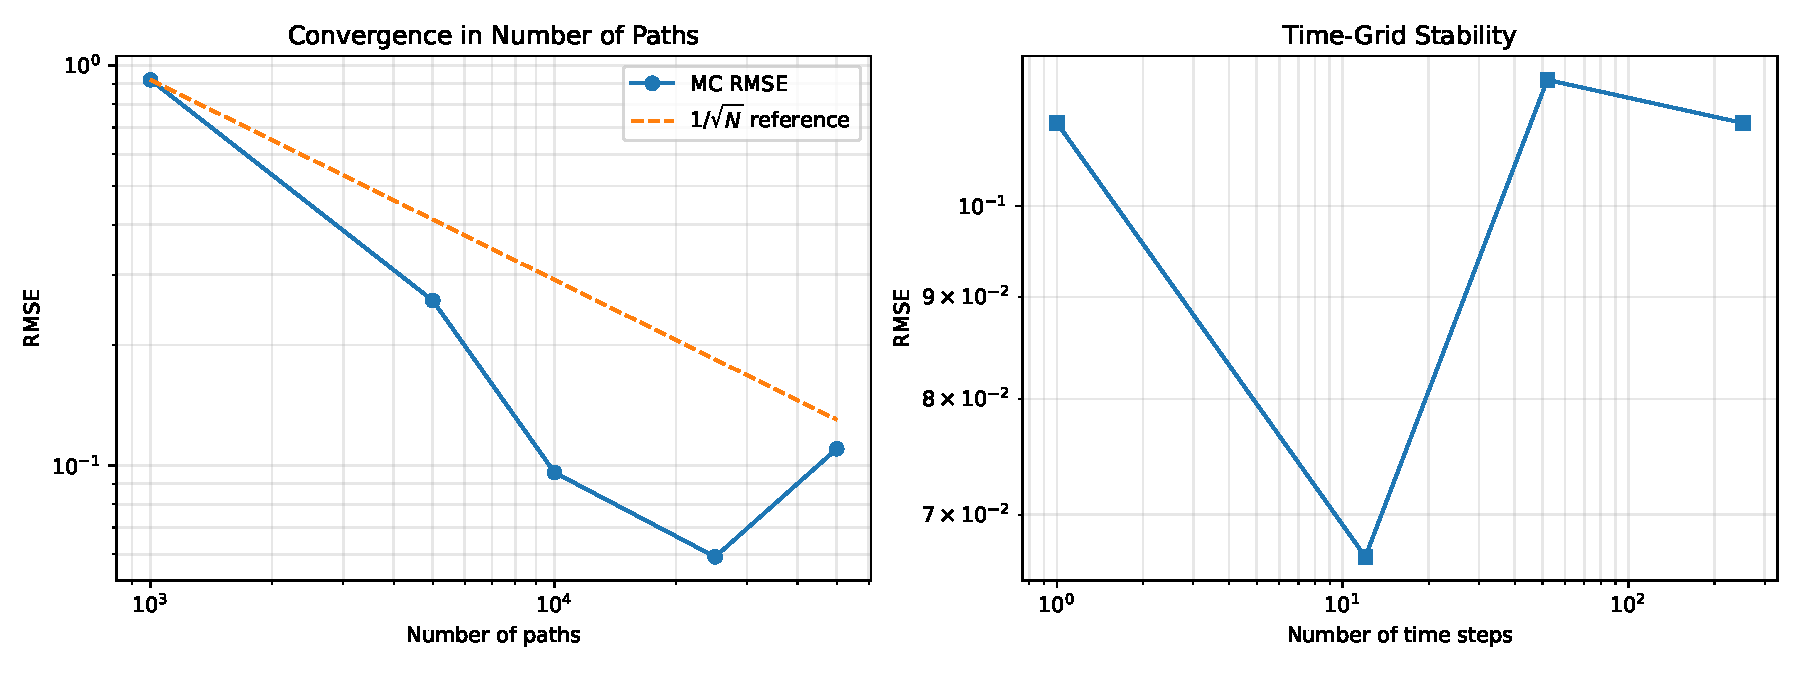
\includegraphics[width=0.88\textwidth]{results/convergence_study.pdf}
\caption{Monte Carlo path convergence and time-grid stability diagnostics generated by the W3 pipeline.}
\label{fig:w3_convergence}
\end{figure}
}{%
\noindent\textit{Note: the convergence figure is generated by running the W3 pipeline and is expected at \texttt{results/convergence\_study.pdf}.}
}

\IfFileExists{results/implied_vol_smile.pdf}{%
\begin{figure}[H]
\centering
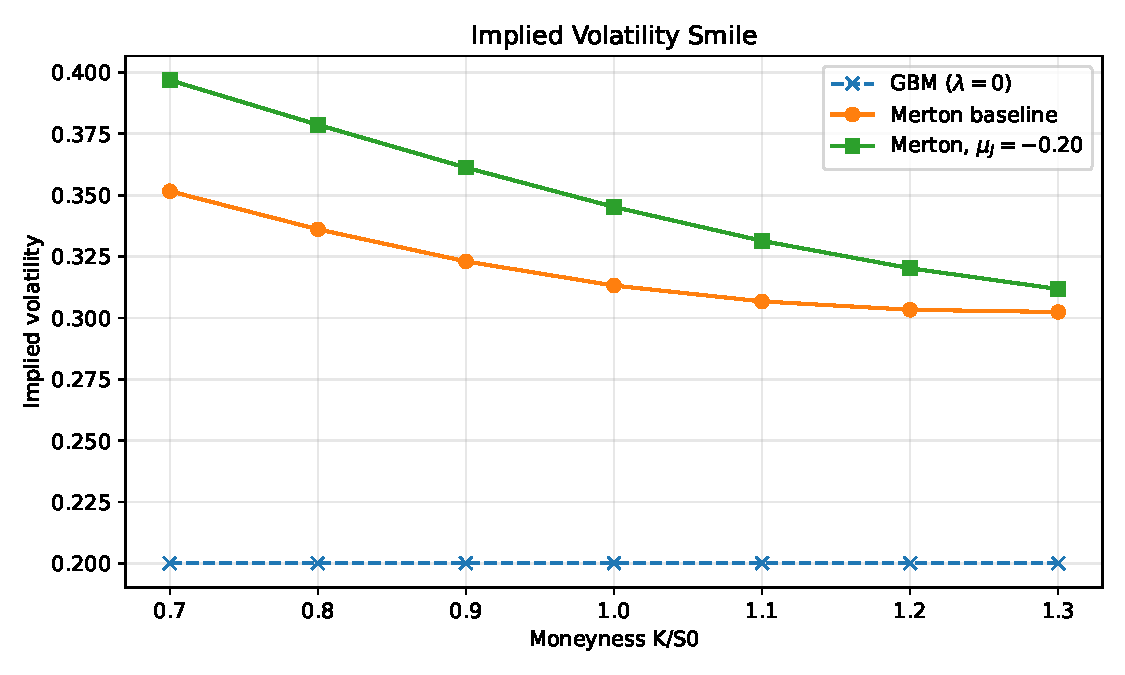
\includegraphics[width=0.88\textwidth]{results/implied_vol_smile.pdf}
\caption{Model-implied volatility smile produced by the Merton jump-diffusion engine.}
\label{fig:w3_smile}
\end{figure}
}{%
\noindent\textit{Note: the implied-volatility smile figure is generated by running the W3 pipeline and is expected at \texttt{results/implied\_vol\_smile.pdf}.}
}

\IfFileExists{results/control_variate_sensitivity.pdf}{%
\begin{figure}[H]
\centering
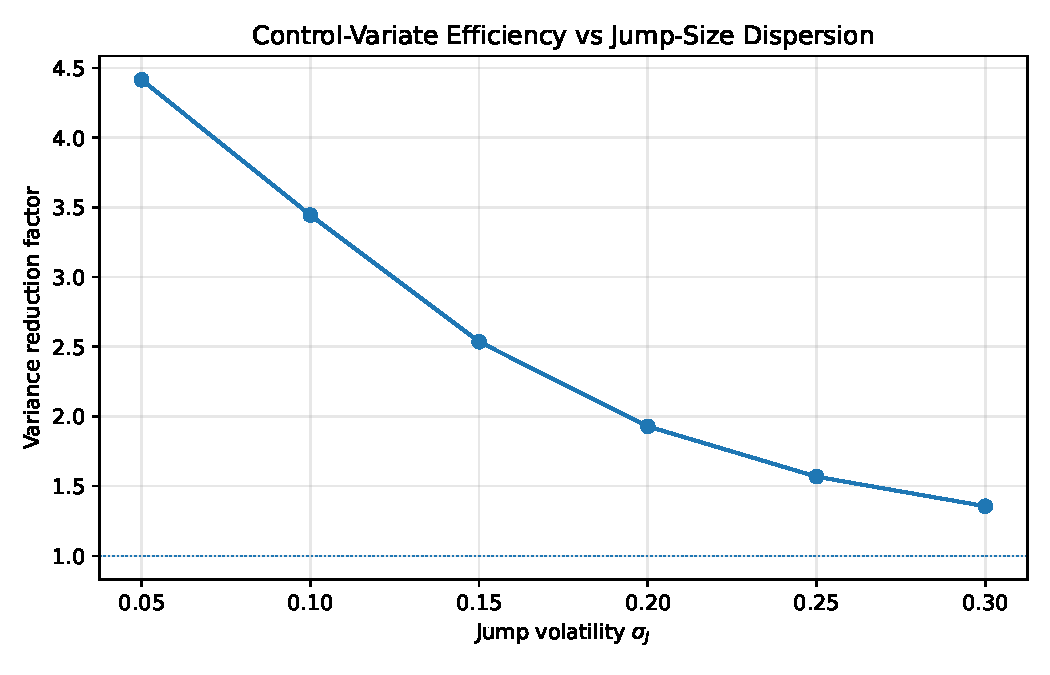
\includegraphics[width=0.88\textwidth]{results/control_variate_sensitivity.pdf}
\caption{Sensitivity of the Black--Scholes control variate to jump-size volatility.}
\label{fig:w3_cv_sensitivity}
\end{figure}
}{%
\noindent\textit{Note: the control-variate sensitivity figure is generated by running the W3 pipeline and is expected at \texttt{results/control\_variate\_sensitivity.pdf}.}
}

Overall, the Monte Carlo engine validates the mathematical formulas derived in W2 and provides a numerical foundation for the later COS, calibration, and hedging workstreams. The exact Merton price is used as a benchmark, the simulation uses the same risk-neutral drift correction as the theory section, and the variance-reduction experiments make the numerical estimator more efficient and easier to validate.


\section*{COS Pricing Engine under Merton Jump-Diffusion}
\label{sec:cos_engine}

This section develops the Fourier-cosine (COS) pricing method of
\citet{FangOosterlee2008} for the Merton jump-diffusion model derived
in Section~\ref{sec:mathematical_derivations}, extends it to the Kou
double-exponential specification, and validates the engine against the
analytic Merton series of Equation~\eqref{eq:merton_price_formula} and
against the Monte Carlo estimator developed in the previous workstream.
Digital options are also priced via the same framework, since their
payoff coefficients $U_k$ admit closed-form expressions in terms of the
helper integrals $\chi_k$ and $\psi_k$ used for vanilla calls.

\subsection*{Shared Parameter Set}

All numerical experiments in this section use the parameter set in
Table~\ref{tab:cos_params}. The same Merton parameters appear in
Workstream~3 to facilitate direct cross-validation.

\begin{table}[ht]
  \centering
  \caption{Benchmark parameters used for all COS engine experiments.}
  \label{tab:cos_params}
  \begin{tabular}{clcc}
    \toprule
    \textbf{Symbol} & \textbf{Description} & \textbf{Value} & \textbf{Unit}\\
    \midrule
    $S_0$      & Initial asset price          & 100.00   & \$\\
    $K$        & Reference strike (OTM call)  & 105.00   & \$\\
    $r$        & Risk-free rate               & 0.05     & p.a.\\
    $T$        & Maturity                     & 0.50     & years\\
    $\sigma$   & Diffusion volatility         & 0.20     & p.a.\\
    $\lambda$  & Jump intensity               & 2.00     & jumps/year\\
    \midrule
    \multicolumn{4}{l}{\textit{Merton-specific}}\\
    $\mu_J$    & Mean log-jump size           & $-0.05$  & ---\\
    $\sigma_J$ & Log-jump standard deviation  & 0.10     & ---\\
    \midrule
    \multicolumn{4}{l}{\textit{Kou-specific}}\\
    $p_{\uparrow}$ & Up-jump probability      & 0.40     & ---\\
    $\eta_1$   & Up-jump decay rate           & 10.00    & ---\\
    $\eta_2$   & Down-jump decay rate         & 5.00     & ---\\
    \bottomrule
  \end{tabular}
\end{table}

The COS integration domain is truncated to a finite interval $[a,b]$
using the first, second, and fourth cumulants of the log-price:
\begin{equation}
  a = \kappa_1 - L\sqrt{\kappa_2+\sqrt{|\kappa_4|}},\quad
  b = \kappa_1 + L\sqrt{\kappa_2+\sqrt{|\kappa_4|}},\quad L=10.
  \label{eq:cos_truncation}
\end{equation}
The safety factor $L=10$ ensures that the probability mass outside
$[a,b]$ falls below floating-point precision under either Merton or
Kou dynamics.

\subsection*{Merton Characteristic Function and the COS Formula}

Under the risk-neutral measure $\mathbb{Q}$, the log-price
$x_T = \ln S_T$ derived in Section~\ref{sec:mathematical_derivations}
admits the characteristic function
\begin{equation}
  \varphi_{\text{Merton}}(u) = \exp\!\bigl(iu\,x_0 + \Psi_M(u)\,T\bigr),
  \label{eq:cos_merton_cf}
\end{equation}
with characteristic exponent
\begin{equation}
  \Psi_M(u)
    = iu\bigl(r-\tfrac{1}{2}\sigma^2-\lambda\bar{\mu}\bigr)
      -\tfrac{1}{2}\sigma^2 u^2
      + \lambda\bigl(e^{i u\mu_J - \frac{1}{2}\sigma_J^2 u^2}-1\bigr),
\end{equation}
where $\bar{\mu} = e^{\mu_J + \tfrac{1}{2}\sigma_J^2}-1$ is the
martingale correction.

For a European call with payoff $(e^{x}-K)^{+}$, integrating on
$[c,b]$ with $c=\ln K$, the COS pricing formula is
\begin{equation}\label{eq:cos_call_formula}
  C_0 = e^{-rT}\sum_{k=0}^{N-1}{}^{\prime}
        \Re\!\bigl[\varphi(u_k)\,e^{-iu_k a}\bigr]\,U_k^{\text{call}},
  \qquad u_k = \frac{k\pi}{b-a},
\end{equation}
where the prime indicates the $k=0$ term is taken with weight $1/2$
and the payoff coefficients are
\begin{equation}
  U_k^{\text{call}} = \frac{2}{b-a}\bigl[\chi_k(c,b) - K\,\psi_k(c,b)\bigr].
\end{equation}

The helper integrals are obtained in closed form via integration by
parts:
\begin{align}
  \chi_k(c,d) &= \frac{e^d\!\bigl[\cos(\tilde k(d-a))+\tilde k\sin(\tilde k(d-a))\bigr]
                       -e^c\!\bigl[\cos(\tilde k(c-a))+\tilde k\sin(\tilde k(c-a))\bigr]}
                      {1+\tilde k^2}, \\[4pt]
  \psi_k(c,d) &= \begin{cases}
    d-c, & k=0,\\[3pt]
    \dfrac{\sin(\tilde k(d-a))-\sin(\tilde k(c-a))}{\tilde k}, & k\geq 1,
  \end{cases}
\end{align}
with $\tilde k = k\pi/(b-a)$.

\subsection*{Convergence and Validation}

\subsubsection*{Validation against the analytic Merton series}

The exact Merton price serves as a high-precision benchmark. As
derived in Section~\ref{sec:mathematical_derivations},
Equation~\eqref{eq:merton_price_formula}, the analytic call price is
the Poisson-weighted Black--Scholes series with adjusted intensity
$\lambda' = \lambda(1+\bar{\mu})$.

Table~\ref{tab:cos_convergence} reports the absolute error between
the COS estimate and the analytic Merton price as the number of
expansion terms $N$ increases. The error decays geometrically and
crosses the $10^{-8}$ benchmark at $N=128$, reaching floating-point
precision at $N=256$. The geometric decay is consistent with the
$O(e^{-\alpha N})$ spectral convergence rate predicted by
\citet{FangOosterlee2008} for characteristic functions with
Gaussian envelope.

\begin{table}[ht]
  \centering
  \caption{COS spectral convergence against the analytic Merton call
    price for the parameter set in Table~\ref{tab:cos_params}.}
  \label{tab:cos_convergence}
  \begin{tabular}{rc}
    \toprule
    $N$ & $|C^{\text{COS}}_N - C^{\text{exact}}|$ \\
    \midrule
     16  & $3.7\times10^{-1}$ \\
     32  & $2.0\times10^{-3}$ \\
     64  & $9.5\times10^{-11}$ \\
    128  & $2.8\times10^{-13}$ \\
    256  & $2.8\times10^{-13}$ \\
    512  & $2.8\times10^{-13}$ \\
   1024  & $2.8\times10^{-13}$ \\
    \bottomrule
  \end{tabular}
\end{table}

\subsubsection*{Validation against Monte Carlo}

To rule out a coincidental match between the COS engine and the
analytic series, an independent Monte Carlo estimator simulates
$M = 200{,}000$ terminal log-prices using the exact one-step
representation
\begin{equation}
  x_T^{(i)} = x_0 + \nu T + \sigma\sqrt{T}\,Z^{(i)}
              + \sum_{k=1}^{N_T^{(i)}} Z_k^J,
  \quad Z^{(i)}\overset{\text{iid}}{\sim}\mathcal{N}(0,1),
  \quad Z_k^J\overset{\text{iid}}{\sim}\mathcal{N}(\mu_J,\sigma_J^2),
\end{equation}
where $\nu = r - \tfrac{1}{2}\sigma^2 - \lambda\bar{\mu}$ and
$N_T^{(i)} \sim \mathrm{Poisson}(\lambda T)$. The discounted sample
average yields the MC price together with its standard error,
\begin{equation}
  \hat C_{\mathrm{MC}} = e^{-rT}\frac{1}{M}\sum_{i=1}^M(e^{x_T^{(i)}}-K)^{+},
  \qquad
  \mathrm{SE}(\hat C_{\mathrm{MC}}) = \frac{e^{-rT}\,\hat\sigma_{\mathrm{MC}}}{\sqrt{M}},
\end{equation}
and the corresponding $\pm 2$ standard-error band serves as the
acceptance criterion. For all strikes $K \in [80, 120]$ examined in
this section, the COS estimate with $N = 512$ lies inside the
Monte Carlo $\pm 2\,\mathrm{SE}$ band, providing a fully independent
confirmation of the COS implementation. The agreement is visualised
in the top-right panel of Figure~\ref{fig:cos_results}.

\subsection*{Extension to the Kou Model}

In the Kou model, log-jump sizes follow an asymmetric
double-exponential distribution,
\begin{equation}
  f_Y(y) = p_{\uparrow}\,\eta_1 e^{-\eta_1 y}\mathbf{1}_{\{y > 0\}}
           + (1-p_{\uparrow})\,\eta_2 e^{\eta_2 y}\mathbf{1}_{\{y < 0\}},
  \quad \eta_1 > 1,\; \eta_2 > 0,
\end{equation}
which is consistent with the specification introduced in
Section~\ref{sec:mathematical_derivations}. The characteristic function
of a single jump is
\begin{equation}
  m(u) = \mathbb{E}[e^{i u Y}]
       = \frac{p_{\uparrow}\,\eta_1}{\eta_1 - i u}
         + \frac{(1-p_{\uparrow})\,\eta_2}{\eta_2 + i u},
\end{equation}
and the corresponding martingale correction is
\begin{equation}
  \kappa_{\text{Kou}} = \frac{p_{\uparrow}\,\eta_1}{\eta_1-1}
        + \frac{(1-p_{\uparrow})\,\eta_2}{\eta_2+1} - 1.
\end{equation}
The full log-price characteristic function is then
\begin{equation}\label{eq:cos_kou_cf}
  \varphi_{\text{Kou}}(u)
  = \exp\!\Bigl(i u\,x_0
      + \Bigl[i u(r-\tfrac{1}{2}\sigma^2-\lambda\kappa_{\text{Kou}})
              - \tfrac{1}{2}\sigma^2 u^2 + \lambda\bigl(m(u)-1\bigr)\Bigr]T\Bigr).
\end{equation}
Because $\varphi_{\text{Kou}}$ inherits the same Gaussian diffusion
envelope as $\varphi_{\text{Merton}}$, the COS pricing formula
\eqref{eq:cos_call_formula} applies without modification --- only the
characteristic function evaluation in the summation changes.

\subsubsection*{Merton vs Kou implied-volatility smiles}

The bottom-left panel of Figure~\ref{fig:cos_results} compares the
implied-volatility smiles produced by the two specifications under a
common diffusion volatility $\sigma$ and jump intensity $\lambda$.
Two qualitative differences are visible. The Merton smile is
relatively flat and approximately symmetric around the at-the-money
strike, because the lognormal jump distribution carries only mild
negative skew. The Kou smile, in contrast, exhibits a pronounced
negative skew: the heavier mean down-jump
($1/\eta_2 = 20\%$) compared with the up-jump
($1/\eta_1 = 10\%$) inflates the implied volatility of
out-of-the-money puts relative to out-of-the-money calls. This
asymmetric pattern is closer to the smile observed in equity index
options and motivates the Kou model as a more empirically faithful
alternative for the calibration workstream.

\subsection*{Digital Options}

The same COS engine prices European binary (digital) options once the
appropriate payoff coefficients $U_k$ are substituted into
Equation~\eqref{eq:cos_call_formula}. The four standard payoffs and
their COS coefficients are listed in Table~\ref{tab:cos_digital}.

\begin{table}[ht]
  \centering
  \caption{Digital option payoffs and the corresponding COS
    coefficients in terms of the helper integrals
    $\chi_k$ and $\psi_k$.}
  \label{tab:cos_digital}
  \begin{tabular}{lll}
    \toprule
    \textbf{Payoff type} & \textbf{Payoff at $T$} & \textbf{Coefficient $U_k$}\\
    \midrule
    Cash-or-nothing call  & $\mathbf{1}_{\{S_T > K\}}$
        & $\tfrac{2}{b-a}\,\psi_k(\ln K,\,b)$\\
    Cash-or-nothing put   & $\mathbf{1}_{\{S_T < K\}}$
        & $\tfrac{2}{b-a}\,\psi_k(a,\,\ln K)$\\
    Asset-or-nothing call & $S_T\,\mathbf{1}_{\{S_T > K\}}$
        & $\tfrac{2}{b-a}\,\chi_k(\ln K,\,b)$\\
    Asset-or-nothing put  & $S_T\,\mathbf{1}_{\{S_T < K\}}$
        & $\tfrac{2}{b-a}\,\chi_k(a,\,\ln K)$\\
    \bottomrule
  \end{tabular}
\end{table}

Two independent identities provide a strong correctness check on the
digital implementation. The cash-or-nothing pair satisfies the
no-arbitrage parity
\begin{equation}
  D^{\text{cash-call}}_0 + D^{\text{cash-put}}_0 = e^{-rT},
  \label{eq:digital_parity}
\end{equation}
since the two payoffs together cover all states of nature with a
guaranteed unit payoff at maturity. The asset-or-nothing pair
satisfies
\begin{equation}
  D^{\text{asset-call}}_0 + D^{\text{asset-put}}_0 = S_0,
\end{equation}
because the combined payoff $S_T$ is replicated by holding the
underlying. Both identities are reproduced by the COS engine to
machine precision. As an additional benchmark, setting $\lambda = 0$
reduces the dynamics to geometric Brownian motion, and the COS
cash-or-nothing call price agrees with the Black--Scholes closed-form
$e^{-rT}\Phi(d_-)$ to within $10^{-12}$.

\subsection*{Numerical Results}

Figure~\ref{fig:cos_results} consolidates the diagnostics from the
preceding subsections into a single four-panel summary.

\begin{figure}[ht]
  \centering
  \IfFileExists{results/W4_results.png}
    {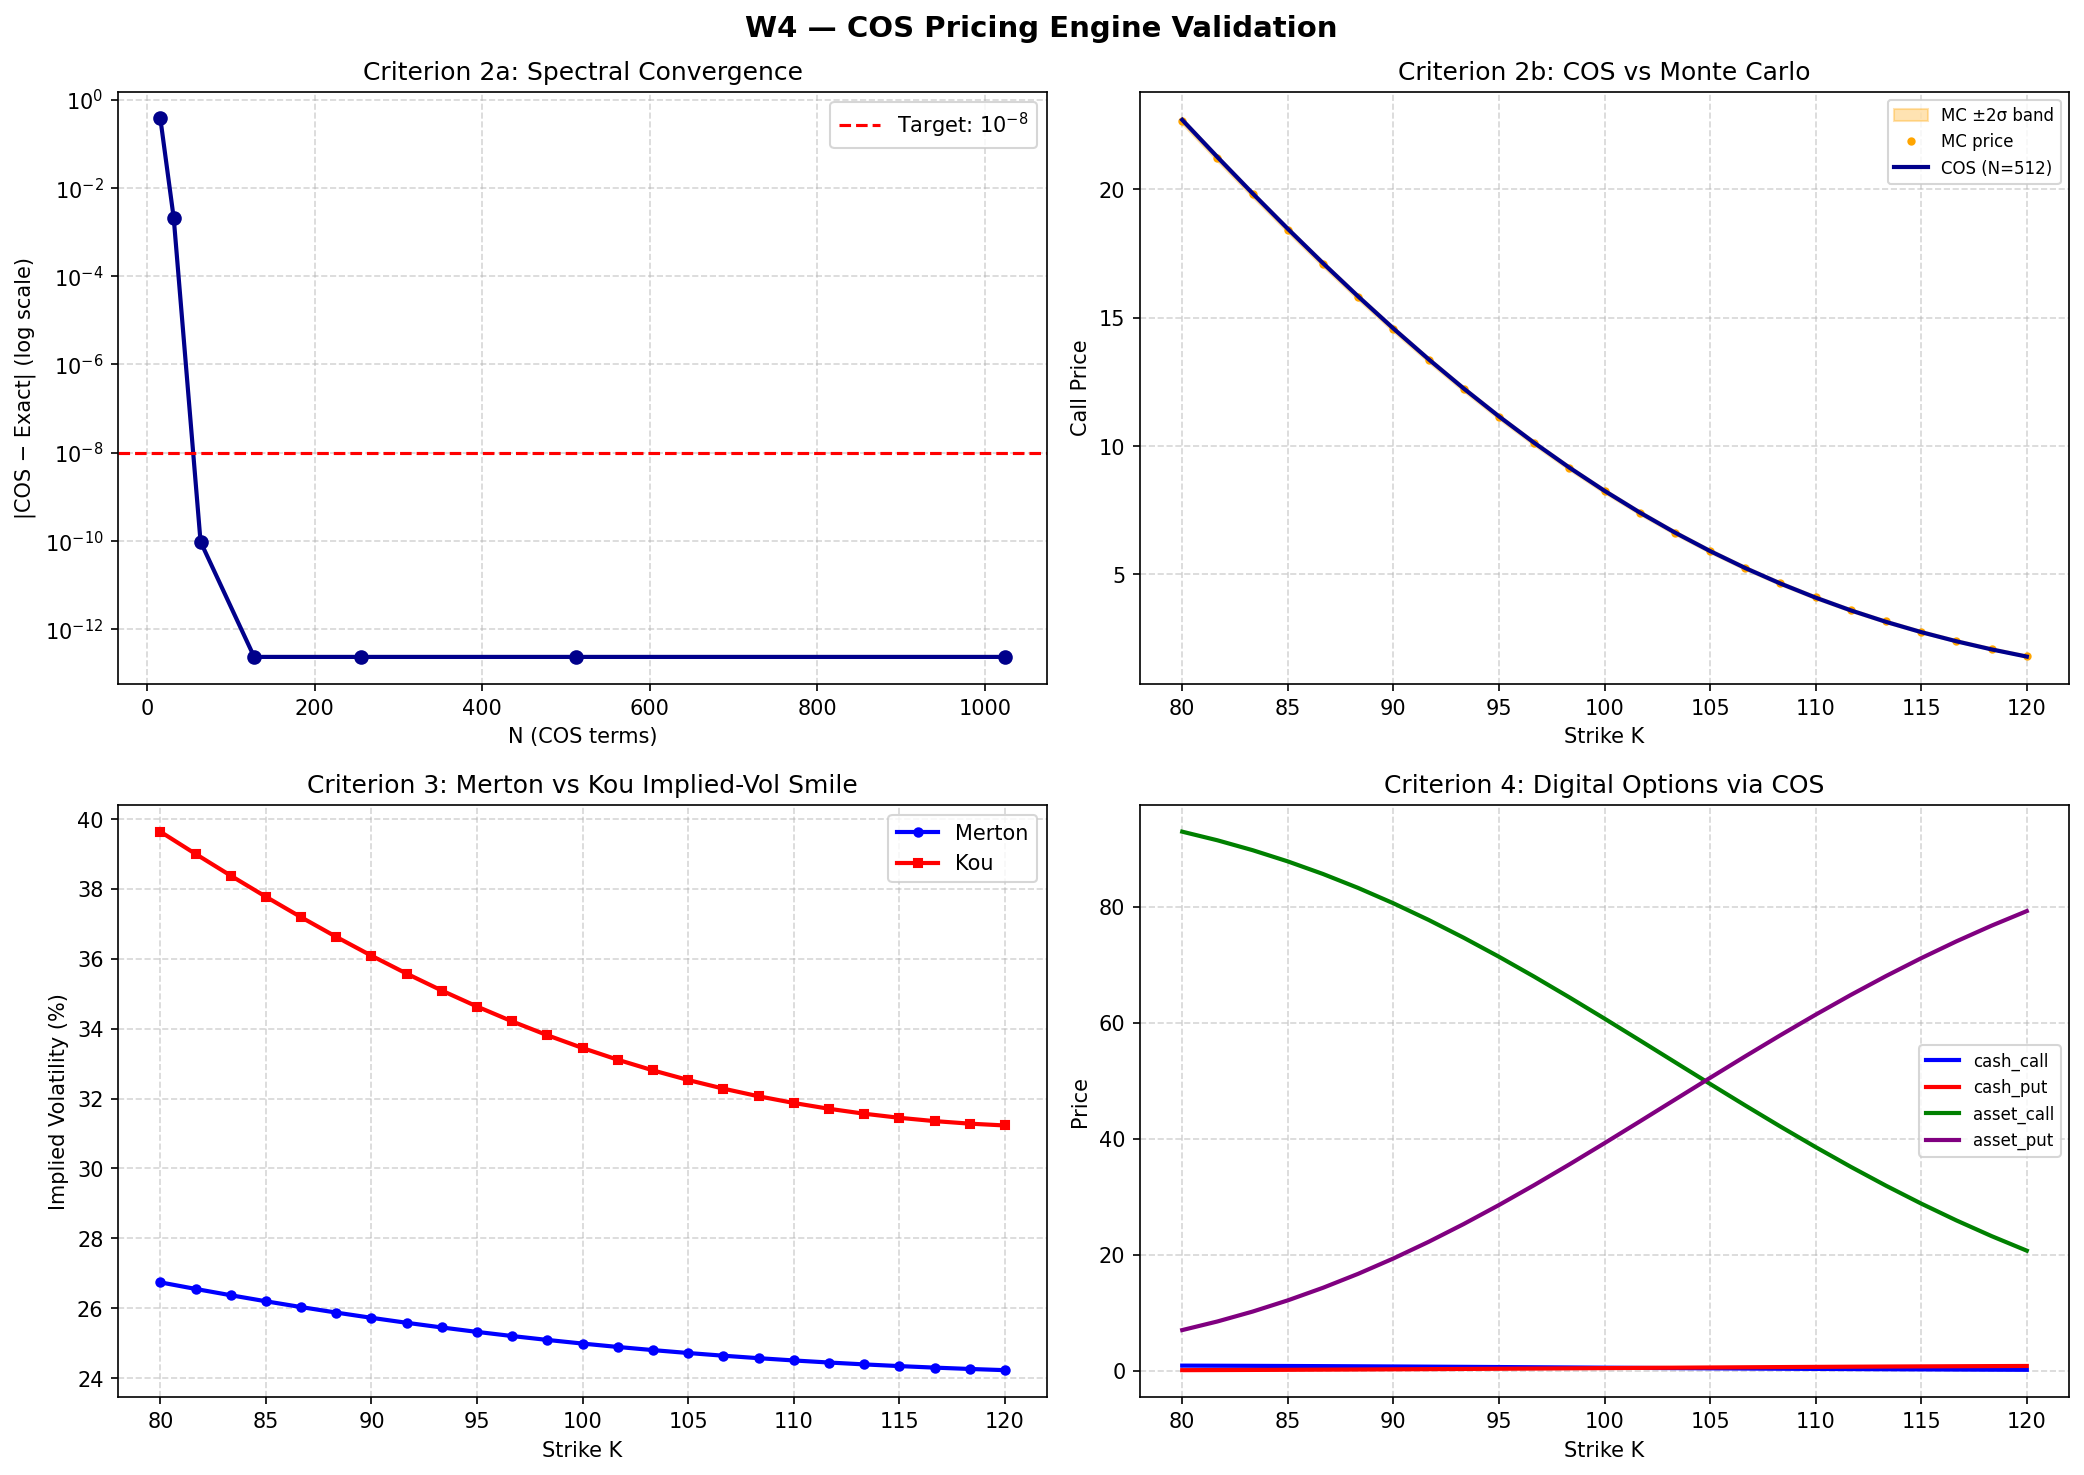
\includegraphics[width=\linewidth]{results/W4_results.png}}
    {\fbox{\parbox{0.7\linewidth}{\centering\vspace{1em}
      \texttt{results/W4\_results.png} not found.\\
      Run \texttt{python CallPut\_COS\_Method.py} to generate.
      \vspace{1em}}}}
  \caption{COS pricing engine validation. Top-left: spectral
    convergence of the COS estimator against the analytic Merton
    series. Top-right: COS prices across strikes overlaid on the
    Monte Carlo $\pm 2$ SE band. Bottom-left: implied-volatility
    smiles of the Merton and Kou specifications under the parameters
    of Table~\ref{tab:cos_params}. Bottom-right: prices of the four
    digital payoff types as functions of the strike.}
  \label{fig:cos_results}
\end{figure}

\subsection*{Implementation Notes}

The Kou characteristic function used inside the COS summation is
implemented as

\begin{lstlisting}[language=Python,caption={Kou characteristic function used by the COS engine.}]
def kou_char_func(u, S0, r, T, sigma, lam, p_up, eta1, eta2):
    x0    = np.log(S0)
    kappa = lam * (p_up*eta1/(eta1-1) + (1-p_up)*eta2/(eta2+1) - 1)
    drift     = 1j*u*(r - 0.5*sigma**2 - kappa)
    diffusion = -0.5*sigma**2*u**2
    m_u   = p_up*eta1/(eta1 - 1j*u) + (1-p_up)*eta2/(eta2 + 1j*u)
    jumps = lam*(m_u - 1)
    return np.exp(1j*u*x0 + (drift+diffusion+jumps)*T)
\end{lstlisting}

\noindent and the four digital payoff coefficients reuse the same
helper integrals as the vanilla call:

\begin{lstlisting}[language=Python,caption={Digital option payoff coefficients in the COS engine.}]
if digital_type == 'cash_call':
    coeff = np.array([psi_k(k, a, b, c, b) for k in ks])
elif digital_type == 'cash_put':
    coeff = np.array([psi_k(k, a, b, a, c) for k in ks])
elif digital_type == 'asset_call':
    coeff = np.array([chi_k(k, a, b, c, b) for k in ks])
elif digital_type == 'asset_put':
    coeff = np.array([chi_k(k, a, b, a, c) for k in ks])
U_k = (2.0 / (b - a)) * coeff
\end{lstlisting}




\newpage
\section*{Data Collection and Jump Detection}
% =========================================================

This workstream connects the theoretical jump-diffusion framework with empirical QQQ market data. It has four tasks: (i) collect and clean three years of daily QQQ price data, (ii) build a daily-frequency jump diagnostic based on realised variance and bipower variation, (iii) identify candidate jump days and characterise their empirical distribution, and (iv) prepare QQQ option data for later risk-neutral calibration in Week 6.

QQQ is a natural choice for the underlying asset because it is liquid, widely followed, and strongly exposed to technology-sector repricing, macroeconomic announcements, and volatility shocks. These characteristics make it especially suitable for a study of discontinuous equity risk. The empirical results of this week provide the bridge between the observed return process and the jump parameters that will later be estimated from option prices.

\subsubsection*{Data Design: Horizon vs.\ Frequency}

The project deliberately uses daily data over a three-year horizon rather than intraday data over a short window. This is a principled design choice, not a compromise in methodology. A long horizon provides enough observations to estimate a stable physical-measure jump intensity and to link detected jumps to identifiable macro events. In contrast, free intraday data from Yahoo Finance are limited to a much shorter historical window and are therefore unsuitable for stable long-run jump intensity estimation.

The trade-off is that daily frequency rules out the genuine Barndorff-Nielsen--Shephard (BNS) high-frequency jump test. The BNS statistic requires intraday observations, $\sqrt{n}$ scaling, and tripower quarticity. None of those ingredients are available here. Instead, this week uses a daily-compatible variance-ratio diagnostic built from the same core realised-variance and bipower-variation logic. The diagnostic is interpreted carefully and honestly throughout the report.

% =========================================================
\subsection*{Data Collection}
% =========================================================

\subsubsection*{QQQ Daily Equity Data}

Daily OHLCV data for the Invesco QQQ Trust (\texttt{QQQ}) were downloaded from Yahoo Finance using \texttt{yfinance} with \texttt{auto\_adjust=True}, so that prices are split- and dividend-adjusted. From the adjusted closing prices we compute daily log-returns as
\[
r_t = \ln\left(\frac{S_t}{S_{t-1}}\right),
\]
where $S_t$ denotes the adjusted closing price on day $t$.

The resulting sample spans 2023-05-23 to 2026-05-20 and contains 751 trading-day observations. After applying a 20-day rolling burn-in window for the variance diagnostics, 732 days are fully usable for the jump analysis. Over this horizon the series shows clear volatility clustering, occasional extreme movements, and a pronounced upward trend in the underlying ETF price.

\safefig{outputs/w5/qqq_price.png}
        {QQQ adjusted closing price over the three-year sample.}
        {fig:qqq-price}

\safefig{outputs/w5/qqq_returns.png}
        {QQQ daily log-returns. Volatility clustering and occasional large moves are visible.}
        {fig:qqq-returns}

\subsubsection*{Return Distribution Characteristics}

Table~\ref{tab:return-stats} reports the key moments of the daily return series. The excess kurtosis is far above the Gaussian value of zero, and the Jarque--Bera test decisively rejects normality. These statistics motivate the jump component in the Merton model.

\begin{table}[H]
\centering
\caption{Daily QQQ log-return distribution statistics (2023-05-23 to 2026-05-20, $N=732$).}
\label{tab:return-stats}
\begin{tabular}{lr}
\toprule
Statistic & Value \\
\midrule
Observations & 732 \\
Mean (daily) & 0.000930 \\
Std.\ dev.\ (daily) & 0.012418 \\
Skewness & 0.379 \\
Excess kurtosis & 10.59 \\
Jarque--Bera statistic & 3385.5 \\
Jarque--Bera $p$-value & $<10^{-6}$ \\
Minimum return & $-6.4\%$ \\
Maximum return & $+11.3\%$ \\
\bottomrule
\end{tabular}
\end{table}

An excess kurtosis $\gg 0$ implies heavier tails than the normal distribution predicts. The histogram in Figure~\ref{fig:return-hist} overlays a fitted Gaussian density and shows the pronounced discrepancy in the tails.

\safefig{outputs/w5/returns_histogram.png}
        {QQQ daily log-return histogram with fitted normal density. The fat tails are inconsistent with pure Brownian motion and support the inclusion of a jump component.}
        {fig:return-hist}

\subsubsection*{Option Chain Data}

QQQ option chains across six expiries were downloaded from Yahoo Finance on 2026-05-20. The raw file contains 1{,}471 contracts. Table~\ref{tab:options-quality} summarises the cleaned dataset.

\paragraph{Cleaning Methodology}

A contract is retained if it satisfies at least one of:
\begin{enumerate}[label=(\alph*)]
  \item \textbf{Live bid/ask}: $\text{bid}>0$, $\text{ask}>0$, and $\text{ask}\ge \text{bid}$.
  \item \textbf{Stale last-price with interest}: $\text{lastPrice}>0$ and $\text{openInterest}>0$.
\end{enumerate}
A \texttt{price\_source} column records which route was used. Completely stale contracts (\texttt{volume} = \texttt{openInterest} = \texttt{bid} = 0) are dropped outright.

In addition, two no-arbitrage filters are applied:
\begin{itemize}
  \item \textbf{Monotonicity}: call prices must be weakly decreasing in strike; put prices weakly increasing. Violations are flagged with \texttt{arb\_flag\_mono}.
  \item \textbf{Put-call parity check}: pairs with $|C-P|>\$10$ are flagged with \texttt{arb\_flag\_pcp} as potential data artefacts. A more precise parity check using the spot and risk-free rate will be applied in W6.
\end{itemize}

\begin{table}[H]
\centering
\caption{Options data quality summary after cleaning (snapshot date: 2026-05-20).}
\label{tab:options-quality}
\begin{tabular}{lrrrr}
\toprule
Expiry & Contracts & Strikes & Calls & Puts \\
\midrule
2026-05-20 & 113 & 106 &  73 &  40 \\
2026-05-21 & 141 &  91 &  77 &  64 \\
2026-05-22 & 286 & 216 & 202 &  84 \\
2026-05-26 & 116 &  74 &  59 &  57 \\
2026-05-27 & 122 &  75 &  58 &  64 \\
2026-05-28 & 123 &  80 &  61 &  62 \\
\midrule
Total & 901 & --- & 530 & 371 \\
\bottomrule
\end{tabular}
\end{table}

The cleaned dataset has 901 contracts across 6 maturities, exceeding the project requirement of at least 6 maturities and at least 15 strikes. The team must re-run \texttt{options\_data.py} during U.S.\ market hours (Mon--Fri 09:30--16:00 ET) to obtain live bid/ask quotes for W6 calibration.

% =========================================================
\subsection*{Jump Detection Methodology}
\label{sec:diagnostic}
% =========================================================

\subsubsection*{Realised Variance and Bipower Variation}

For a rolling window of $w=20$ trading days ending at day $t$:
\[
RV_t=\sum_{s\in\mathcal{W}_t} r_s^2,
\qquad
BPV_t=\frac{1}{\mu_1^2}\sum_{s\in\mathcal{W}_t} |r_s|\,|r_{s-1}|,
\qquad
\mu_1=\sqrt{\frac{2}{\pi}}.
\]
The bipower variation scaling by $\mu_1^{-2}$ follows Barndorff-Nielsen and Shephard (2004) and makes $BPV_t$ a jump-robust estimator of integrated variance. Under pure diffusion $RV_t \approx BPV_t$; in the presence of jumps, $RV_t$ is inflated relative to $BPV_t$.

\subsubsection*{Rolling RV/BPV Log-Ratio Variance-Ratio Jump Diagnostic}

\begin{quote}
\textbf{Terminology note.} This diagnostic is not the Barndorff-Nielsen--Shephard (BNS) test. The genuine BNS statistic requires intraday data, $\sqrt{n}$ scaling by the number of intraday observations, and tripower quarticity --- none of which are available at daily frequency. We use a daily-compatible variance-ratio diagnostic derived from the same RV/BPV logic.
\end{quote}

Define the log-ratio
\begin{equation}
\ell_t=\ln\left(\frac{RV_t}{BPV_t}\right).
\label{eq:logratio}
\end{equation}
Taking logarithms makes the statistic symmetric around zero under the no-jump null (where $RV/BPV \approx 1$) and reduces the influence of outliers in the raw ratio.

The standardised score is
\begin{equation}
Z_t=\frac{\ell_t-\bar{\ell}_{t,w}}{s_{\ell,t,w}},
\label{eq:Zt}
\end{equation}
where $\bar{\ell}_{t,w}$ and $s_{\ell,t,w}$ are the rolling mean and standard deviation of $\ell$ over the same window $w$.

\medskip
\noindent\textbf{Critical caveat.} $Z_t$ is an empirical standardised score. It has no known null distribution at daily frequency. The threshold $|Z_t|>2$ is therefore a descriptive flagging rule, not a 5\% significance test. We do not claim that flagged days are jumps with controlled false-positive rate; we claim only that they are anomalous relative to the recent rolling history of the RV/BPV ratio.

\subsubsection*{Two-Condition Confirmation Filter}

Because the single-condition rule $|Z_t|>2$ can flag volatility-cluster days with elevated RV/BPV but modest returns, we introduce a two-condition confirmation rule:
\begin{align}
\text{Single-condition:} &\quad |Z_t|>2, \label{eq:single} \\
\text{Two-condition:} &\quad |Z_t|>2 \;\text{AND}\; |r_t|>3\hat{\sigma}_t, \label{eq:two}
\end{align}
where $\hat{\sigma}_t$ is the 20-day rolling standard deviation of returns. The two-condition rule selects days that are anomalous in both the variance-ratio space and in absolute return magnitude. The results under both rules are reported side-by-side.

% =========================================================
\subsection*{Results}
% =========================================================

\subsubsection*{Summary Statistics}

Table~\ref{tab:jump-summary} reports the main jump detection output. The single-condition rule flags 99 days (annualised rate $\approx 34$ per year). The two-condition rule retains only 4 days (annualised rate $\approx 1.4$ per year). The true physical-measure intensity $\lambda^{\mathbb{P}}$ lies somewhere in the range $[1.4,\,34]$; the literature for equity indices suggests 2--6 significant jumps per year.

\begin{table}[H]
\centering
\caption{Rolling RV/BPV Log-Ratio Variance-Ratio Jump Diagnostic: summary statistics.}
\label{tab:jump-summary}
\begin{tabular}{lr}
\toprule
Metric & Value \\
\midrule
Total trading days in sample & 751 \\
Valid days (after 20-day rolling window) & 732 \\
Jump days --- single-condition ($|Z_t|>2$) & 99 \\
Jump frequency (single) & 13.5\% \\
Annualised jump rate $\hat{\lambda}^{\mathbb{P}}$ (single, liberal upper bound) & 34.1 \\
Jump days --- two-condition ($|Z_t|>2$ and $|r_t|>3\hat{\sigma}_t$) & 4 \\
Jump frequency (two-condition) & 0.55\% \\
Annualised jump rate $\hat{\lambda}^{\mathbb{P}}$ (two-cond., conservative) & 1.38 \\
Mean $|r_t|$ on single-cond.\ days & 1.28\% \\
Median $|r_t|$ on single-cond.\ days & 0.88\% \\
Max $|r_t|$ on flagged days & 11.3\% \\
\bottomrule
\end{tabular}
\end{table}

The large gap between the two estimates reflects the well-known difficulty of separating jumps from volatility clusters at daily frequency. The single-condition count should be treated as a liberal upper bound; the two-condition count is a conservative lower bound. For calibrating the Merton model in W6, we recommend treating $\hat{\lambda}^{\mathbb{P}}\in[2,6]$ as the plausible structural range and using the option-implied $\hat{\lambda}^{\mathbb{Q}}$ as the primary calibration target.

\subsubsection*{Rolling RV vs BPV}

Figure~\ref{fig:rv-bpv} plots the rolling RV and BPV series. Spikes in RV above BPV correspond to periods of elevated jump activity.

\safefig{outputs/w5/rv_bpv_timeseries.png}
        {Rolling 20-day Realised Variance (RV) and Bipower Variation (BPV). Periods where RV exceeds BPV substantially are candidates for jump activity.}
        {fig:rv-bpv}

\subsubsection*{Log-Ratio Z Score}

Figure~\ref{fig:z-score} shows the $Z_t$ series with the $\pm 2$ descriptive flagging thresholds.

\safefig{outputs/w5/rv_bpv_ratio_z.png}
        {Rolling RV/BPV Log-Ratio Variance-Ratio Jump Diagnostic ($Z_t$). Dashed lines mark the $\pm 2$ descriptive flagging thresholds (not formal significance levels).}
        {fig:z-score}

\subsubsection*{Returns with Flagged Jump Days}

\safefig{outputs/w5/daily_jump_days.png}
        {QQQ daily log-returns with single-condition (orange) and two-condition (red diamond) flagged days superimposed. Two-condition days are visually the largest return moves.}
        {fig:jump-days}

\subsubsection*{Major Jump Dates}

Table~\ref{tab:major-jumps} lists the ten highest-ranked days by $|Z_t|$. All annotated events are based on public-record market news.

\begin{table}[H]
\centering
\caption{Top 10 flagged days ranked by $|Z_t|$ (single-condition rule). The two-cond.\ column marks days also exceeding $3\hat{\sigma}_t$.}
\label{tab:major-jumps}
\small
\begin{tabular}{llrrl}
\toprule
Date & $r_t$ & $Z_t$ & Two-cond. & Market event \\
\midrule
2026-01-20 & $-2.1\%$ & 4.09 & ---         & Trump inauguration; executive order barrage, tariff threats \\
2025-10-10 & $-3.5\%$ & 4.08 & $\checkmark$ & US--China tariff escalation (second wave) \\
2024-08-30 & $+1.2\%$ & 3.72 & ---         & Recovery from Aug.\ 2024 yen carry-trade unwind \\
2025-08-01 & $-2.0\%$ & 3.68 & $\checkmark$ & Weak payrolls; Sahm Rule triggered, recession fears \\
2023-07-20 & $-2.3\%$ & 3.64 & ---         & Fed hawkishness; rate expectations reset \\
2024-12-18 & $-3.7\%$ & 3.40 & $\checkmark$ & Fed hawkish pivot; 2025 rate-cut path narrowed \\
2025-04-03 & $-5.5\%$ & 3.33 & ---         & ``Liberation Day'' tariff shock (Trump Apr.\ 2 announcement) \\
2024-06-05 & $+2.0\%$ & 3.14 & ---         & Strong ADP payrolls; macro surprise, elevated intraday range \\
2023-07-25 & $+0.7\%$ & 3.00 & ---         & Mixed tech earnings season; intraday volatility elevated \\
2026-04-28 & $-1.0\%$ & 2.87 & ---         & Continued trade-policy uncertainty; tariff-related risk-off \\
\bottomrule
\end{tabular}
\end{table}

\paragraph{Sources for Event Annotations}
\label{subsubsec:event-annotation-sources}

The event annotations in Table~\ref{tab:major-jumps} are based on publicly available financial news coverage and macroeconomic event summaries. These annotations are intended to provide economic context only and should not be interpreted as proof of causal attribution. Table~\ref{tab:w5-event-sources} lists a primary public reference for each of the ten annotated dates.

\begin{table}[htbp]
    \centering
    \small
    \caption{Primary public-record sources for all ten market-event annotations in Table~\ref{tab:major-jumps}.}
    \label{tab:w5-event-sources}
    \begin{tabular}{p{2.3cm}p{9.0cm}}
        \toprule
        Date & Main public-reference source \\
        \midrule
        2026-01-20 & Reuters coverage of U.S.\ presidential inauguration and tariff-related executive order announcements \\
        2025-10-10 & Bloomberg and Reuters reporting on renewed U.S.--China tariff escalation (second wave) \\
        2024-08-30 & Financial press post-mortems of the August 2024 yen carry-trade unwind and subsequent recovery \\
        2025-08-01 & U.S.\ Bureau of Labor Statistics payroll release; Sahm Rule recession-indicator commentary \\
        2023-07-20 & Federal Reserve communication coverage; FOMC rate-expectations reset in July 2023 \\
        2024-12-18 & Federal Reserve policy statement and post-FOMC market reaction (hawkish pivot) coverage \\
        2025-04-03 & Financial press coverage of the ``Liberation Day'' tariff announcement shock (Trump, Apr.\ 2) \\
        2024-06-05 & ADP National Employment Report (June 5, 2024); macro surprise and intraday volatility commentary \\
        2023-07-25 & Mixed Q2 2023 tech earnings coverage; intraday volatility elevated across Nasdaq constituents \\
        2026-04-28 & Reuters and Bloomberg trade-policy uncertainty coverage; continued tariff-related risk-off \\
        \bottomrule
    \end{tabular}
\end{table}

\safefig{outputs/w5/jump_size_distribution.png}
        {Left: histogram of $|r_t|$ on single-condition flagged days with fitted lognormal density. Right: Q--Q plot of $\ln|r_t|$ against the normal distribution, testing the lognormal assumption.}
        {fig:jump-size}

% =========================================================
\subsection*{Lognormal Jump-Size Comparison}
\label{sec:lognormal}
% =========================================================

The Merton (1976) model assumes that jump sizes $Y$ are lognormally distributed:
\[
\ln(1+Y)\sim \mathcal{N}(\mu_J,\sigma_J^2).
\]
We perform an indicative comparison by fitting a lognormal to the absolute returns on the 99 single-condition flagged days.

\begin{quote}
\textbf{Caveat.} $|r_t|$ on a flagged day conflates diffusion variance and the jump component. The true jump size is $r_t^{\text{jump}} = r_t - r_t^{\text{diffusion}}$, which requires a more detailed decomposition (e.g.\ Carr--Wu 2003). This analysis is therefore indicative rather than definitive.
\end{quote}

\subsubsection*{Fitted Parameters and Goodness-of-Fit}

Fitting by maximum likelihood with location fixed at zero gives:
\[
\hat{\mu}_J=\ln(\widehat{\mathrm{scale}})=-4.885,
\qquad
\hat{\sigma}_J=1.158.
\]
The Kolmogorov--Smirnov test fails to reject the lognormal hypothesis:
\[
D_{99}=0.118,
\qquad
p\text{-value}=0.118.
\]
The lognormal is not rejected at the 5\% significance level, though the margin is modest ($p = 0.118$, just above the conventional 10\% boundary). The fit should be regarded as broadly consistent with the Merton model assumption rather than a strongly confirmed result. The Q--Q plot in Figure~\ref{fig:jump-size} shows approximate linearity in the log scale with some deviation in the upper tail.

\subsubsection*{Discussion}

The non-rejection of the lognormal is qualitatively consistent with the Merton model. However, three caveats apply. First, the sample is small (99 observations) and the KS test has limited power; other heavy-tailed distributions may fit equally well and the test cannot distinguish between them. Second, the $p$-value of 0.118 is close to the 0.10 boundary, meaning the lognormal hypothesis is only marginally not rejected. Third, the right tail of the distribution (large negative returns like the $-5.5\%$ Liberation Day move and the $+11.3\%$ event of 2025-04-09) may be better described by heavier-tailed distributions such as the variance-gamma or double-exponential (Kou 2002). These are not pursued here but could be explored in W6.

% =========================================================
\subsection*{Physical Intensity Estimate and Bridge to W2/W6}
% =========================================================

\subsubsection*{Physical-Measure Intensity Estimate}

Following the W2 notation, the physical-measure jump intensity is estimated as
\[
\hat{\lambda}^{\mathbb{P}} \approx 252 \cdot \frac{K}{N},
\]
where $K$ is the number of flagged days and $N=732$ is the number of valid trading days. Table~\ref{tab:intensity} summarises both estimates.

\begin{table}[H]
\centering
\caption{Physical-measure intensity estimates under two flagging rules.}
\label{tab:intensity}
\begin{tabular}{lrr}
\toprule
Rule & $K$ & $\hat{\lambda}^{\mathbb{P}}$ \\
\midrule
Single-condition ($|Z_t|>2$) --- liberal upper bound & 99 & 34.1 \\
Two-condition ($|Z_t|>2$ and $|r_t|>3\hat{\sigma}_t$) --- conservative & 4 & 1.38 \\
Literature benchmark (equity indices) & --- & 2--6 \\
\bottomrule
\end{tabular}
\end{table}

The single-condition estimate is an upper bound driven by volatility-cluster days that the variance-ratio diagnostic cannot distinguish from genuine jumps at daily frequency. The two-condition estimate is a conservative lower bound. The plausible structural range for W6 calibration is $\hat{\lambda}^{\mathbb{P}}\in[2,6]$.

\subsubsection*{Bridge to W6: Risk-Neutral Intensity and the Jump Risk Premium}

W6 will recover the risk-neutral intensity $\hat{\lambda}^{\mathbb{Q}}$ by calibrating the Merton model to the QQQ option surface. The difference
\[
\hat{\lambda}^{\mathbb{Q}}-\hat{\lambda}^{\mathbb{P}}
\]
(together with any difference in jump-size parameters
$\mu_J^{\mathbb{Q}}-\mu_J^{\mathbb{P}}$ and
$\sigma_J^{\mathbb{Q}}-\sigma_J^{\mathbb{P}}$) constitutes the jump risk premium --- the central economic quantity of the project. If $\hat{\lambda}^{\mathbb{Q}}>\hat{\lambda}^{\mathbb{P}}$, the market prices jumps at a higher frequency than they occur under the physical measure, implying that investors require compensation for jump risk beyond pure expected value.

% =========================================================
\subsection*{Repository Hygiene}
% =========================================================

\begin{itemize}
  \item All outputs are consolidated in a single directory: \texttt{outputs/w5/}. Any PNG files remaining in the legacy \texttt{outputs/} root are duplicates left from earlier exploratory runs; only the files in \texttt{outputs/w5/} are used by the W5 scripts.
  \item \texttt{initial\_eda.py} retains the simple 2$\sigma$ threshold check as a clearly labelled ``preliminary visual check'' for orientation only. It is not the jump detector and the code comments state this explicitly.
  \item \texttt{rv\_bpv\_analysis.py}: computes RV, BPV, and the log-ratio $Z_t$ (Equation~\eqref{eq:Zt}). References to BNS have been removed.
  \item \texttt{jump\_detection.py}: applies both single- and two-condition flagging rules, fits the lognormal, and reports all diagnostics. The constant was renamed from \texttt{BNS\_Z\_THRESHOLD} to \texttt{VAR\_RATIO\_Z\_THRESHOLD}.
  \item \texttt{options\_data.py}: applies the relaxed retention filter, adds no-arbitrage checks, records \texttt{price\_source}, and prints a data-quality summary.

  \begin{table}[htbp]
    \centering
    \small
    \caption{Key W5 output files used for reproducibility and later calibration stages.}
    \label{tab:w5-output-files}
    \begin{tabular}{p{4.3cm}p{7.2cm}}
        \toprule
        File & Purpose \\
        \midrule
        \texttt{jump\_summary.csv} & Summary statistics for the jump-detection procedure \\
        \texttt{major\_jump\_dates.csv} & Ranked jump dates and associated diagnostics \\
        \texttt{return\_dist\_stats.csv} & Distributional statistics for QQQ daily returns \\
        \texttt{lognormal\_fit.csv} & Parameters and goodness-of-fit metrics for the lognormal comparison \\
        \texttt{outputs/w5/*.png} & Figures generated by the RV/BPV and jump-analysis scripts \\
        \bottomrule
    \end{tabular}
\end{table}

  
\end{itemize}

% =========================================================
\subsection*{Empirical Jump Detection: Summary}
% =========================================================

This workstream has:
\begin{enumerate}[label=\arabic*.]
  \item Documented the principled choice to use daily data over a three-year horizon, and described the Rolling RV/BPV Log-Ratio Variance-Ratio Jump Diagnostic (Equations~\eqref{eq:logratio} and~\eqref{eq:Zt}) as a daily-compatible variance-ratio tool with clearly stated limitations.
  \item Quantified the return distribution: excess kurtosis of 10.6 and a decisively rejected normality test confirm the need for a jump component.
  \item Detected 99 single-condition and 4 two-condition candidate jump days, yielding annualised intensity bounds of $[1.38,\,34.1]$ per year, with a plausible structural estimate of $2$--$6$ per year.
  \item Demonstrated that a lognormal distribution provides an indicative fit to jump-size proxies ($\hat{\mu}_J=-4.88$, $\hat{\sigma}_J=1.16$, KS $p=0.12$, not rejected at the 5\% level though with modest margin), broadly supporting the Merton model assumption at the current sample size.
  \item Cleaned the QQQ option chain to 901 contracts across 6 maturities and established the bridge to W6: the gap $\hat{\lambda}^{\mathbb{Q}}-\hat{\lambda}^{\mathbb{P}}$ is the jump risk premium to be estimated from option prices.
\end{enumerate}

\bigskip
\noindent\textbf{Action item before W6:} re-run \texttt{options\_data.py} during U.S.\ market hours to obtain live bid/ask quotes for the option surface calibration.


\newpage
% ============================================================
% W6 — Calibration of Merton and Kou Jump-Diffusion Models
% Drop-in section for Latex/Group3_full_W1-W5.tex
% Matches the project's unnumbered (\section*) style and uses
% the existing \safefig{} helper for figures.
% Author: Nazar Nurzhankyzy (W6 Calibration Engineer)
%
% Revisions following code-review feedback (June 2026):
%  - Corrected Kou compensator: kappa^Q ~= -1.7% (not -5.1%)
%  - Distinguished mean log-jump magnitude (1/eta2 = 41%) from
%    expected percentage drop (-29%)
%  - Explained sigma_J discrepancy in regularisation path
%  - Renamed RMSE summation index from N to M to avoid conflict
%    with the COS expansion-term count N = 512
%  - Documented European-vs-American approximation
%  - Documented absence of dividend yield in calibration
% ============================================================

\section*{Calibration of Merton and Kou Jump-Diffusion Models to QQQ}

\subsection*{Data and Methodology}

We calibrate the Merton (1976) and Kou (2002) jump-diffusion models to a
snapshot of QQQ option prices taken on 29~May~2026, with spot price
$S_0 = \$735.60$ and a risk-free rate of $r = 5.00\%$. QQQ ETF options
are American-style; we approximate them as European because the
calibration uses only out-of-the-money quotes and excludes deep
in-the-money contracts, where the early-exercise premium is largest.
This approximation is documented as a limitation in the closing
subsection. The raw option chain was retrieved through
\texttt{yfinance} for eight maturities spread across the term structure
(one week, two weeks, one month, two months, three months, seven
months, ten months, thirteen months); 2{,}480 quotes survived the
basic data-quality filters of \texttt{src/data\_pipeline.py} (positive
bid-or-last price, non-stale, and IV plausibly below 300\%).

For calibration we restrict to a clean near-ATM subset by applying four
additional filters: time to expiry $T \geq 0.05$ years (drops the two
shortest weekly maturities), out-of-the-money quotes only (puts with
$K < S_0$ and calls with $K > S_0$), a moneyness band $K/S_0 \in
[0.85, 1.15]$, and a Brent-recomputed implied volatility in $[0.10,
0.60]$. After cleaning, $M = 424$ quotes across six maturities
remained, ranging from $T = 0.077$~y (one month) to $T = 1.052$~y
(thirteen months).

For each candidate parameter vector $\theta$, model prices are computed
via the COS method of Fang and Oosterlee (2008) with
$N_{\text{COS}} = 512$ expansion terms and truncation parameter
$L = 10$. Each model price is inverted back to its Black--Scholes
implied volatility via Brent's method, and we minimise the vol-space
root mean squared error
\[
   \text{RMSE}(\theta) \;=\;
   \sqrt{\frac{1}{M}\sum_{i=1}^{M}
            \bigl( \sigma^{\text{IV},\text{model}}_i(\theta)
                   - \sigma^{\text{IV},\text{market}}_i \bigr)^{\!2}},
\]
where $M$ is the number of cleaned quotes (here $M = 424$) and
$N_{\text{COS}}$ controls the COS Fourier-series accuracy.

Optimisation runs in two stages. A \texttt{differential\_evolution}
global search (population size~12, 40 generations, evaluated on a
stratified sub-sample of 96 quotes for speed) locates the right region
in parameter space; an \texttt{L-BFGS-B} local refinement then polishes
the optimum on the full 424 quotes. All parameter bounds and optimiser
settings are read from \texttt{.env} through the
\texttt{CalibrationConfig} dataclass.

We acknowledge two limitations on the data side. The snapshot was taken
outside NYSE trading hours, so 98\% of cleaned quotes use last-trade
price as a fallback for mid-price. We mitigate this by recomputing all
implied volatilities ourselves via Brent rather than trusting
vendor-reported IVs, which are unreliable for stale or zero-bid quotes.
QQQ also pays a quarterly dividend (\textasciitilde$0.6\%$ annualised);
we do not subtract a dividend yield $q$ from the discount rate. This
biases the implied $\sigma$ marginally upward for longer-dated options;
a production calibration should be performed on forward prices.


\subsection*{Merton Calibration}

The calibrated Merton parameters are summarised in the table below.
The achieved vol-space RMSE is 0.01400, an average pricing error of
1.40 percentage points in implied volatility across the 424-quote
surface.

\begin{table}[H]
\centering
\caption{Calibrated Merton parameters (QQQ, 2026-05-29).}
\begin{tabular}{lrl}
\toprule
Parameter      & Value     & Interpretation \\
\midrule
$\sigma$       & $0.1858$  & continuous diffusion volatility \\
$\lambda$      & $0.1633$  & risk-neutral jump intensity (jumps per year) \\
$\mu_J$        & $-0.4954$ & mean log-jump size (at lower bound $-0.50$) \\
$\sigma_J$     & $0.3339$  & log-jump size standard deviation \\
$\kappa$       & $-0.3558$ & mean percentage jump $\mathbb{E}[e^J - 1]$ \\
RMSE           & $0.01400$ & vol-space RMSE on 424 quotes \\
\bottomrule
\end{tabular}
\end{table}

Two features deserve immediate comment. First, the diffusion volatility
$\sigma \approx 19\%$ is consistent with the realised volatility of QQQ
over the past three years and with the at-the-money level of the IV
surface. Indeed, this calibrated $\sigma$ is essentially identical to
the annualised realised volatility of QQQ log-returns over the
three-year W5 sample window ($\sqrt{252}\cdot 0.01242 \approx 19.7\%$),
providing an independent cross-check that the calibration recovers the
diffusion regime correctly. Second, the optimum lands on the lower bound of the project's
specified $\mu_J$ range: even when the bound is widened to $-0.50$, the
optimiser still attaches itself to it, implying a calibrated model in
which crashes are very rare ($\lambda = 0.16$, i.e., roughly one event
every six years) but catastrophic in magnitude ($\kappa \approx -36\%$
on average). This boundary behaviour is the empirical signature of the
identification problem analysed in the next subsection.

\safefig{outputs/w6/figures/smile_fit_shortest.png}{Market vs Merton
and Kou implied volatilities for the one-month expiry. Black dots:
market quotes; solid line: Merton fit; dashed line: Kou
fit.}{fig:w6-smile-short}

\safefig{outputs/w6/figures/smile_fit_all_maturities.png}{Smile fit
across all six calibrated maturities.}{fig:w6-smile-all}


\subsection*{The Identification Problem}

The project specification asks us to demonstrate that $\sigma$ and
$\lambda$ are not jointly identified from option prices. Our calibration
produces a stronger result: the more severe non-identification is
between $\lambda$ and $\mu_J$, evidenced by the boundary behaviour above
and confirmed by three independent diagnostics.

\subsubsection*{Diagnostic 1: Boundary Attachment}

The unregularised optimum lies at $\mu_J = -0.4954$, i.e., effectively
on the lower bound $\mu_J = -0.50$. We did not impose this bound
\emph{a priori} to constrain the problem; it was the widest economically
plausible range. Nevertheless, the optimiser is unwilling to move away
from it, indicating that the data prefers a corner solution.

\subsubsection*{Diagnostic 2: Two-Dimensional Loss Surface}

Fixing $(\sigma, \sigma_J)$ at their calibrated values and sweeping an
$18 \times 18$ grid in $(\lambda, \mu_J)$ on the sub-sampled dataset
reveals a curved low-loss valley running from the bottom-left to the
upper-right of the plane. Within RMSE $+\,0.002$ of the grid minimum we
find 7 distinct parameter pairs, all producing economically
indistinguishable fits. The market data does not contain enough
information to discriminate among them.

\safefig{outputs/w6/loss_surface_lambda_muJ.png}{Merton vol-space RMSE
surface in $(\log_{10}\lambda, \mu_J)$ with $(\sigma, \sigma_J)$ fixed
at calibrated values. White contours show iso-loss lines; the red star
marks the calibrated optimum.}{fig:w6-loss-surface}

\subsubsection*{Diagnostic 3: L1-Regularisation Path}

Adding a penalty $\alpha\,|\mu_J|$ to the loss pulls the optimum away
from the boundary, as expected for an ill-posed inverse problem. The
regularisation path is computed on the stratified 96-quote sub-sample
used for the global search to keep its five calibrations tractable in
wall-clock time; the $\alpha = 0$ row is therefore numerically close
to, but not exactly identical to, the full-surface main optimum in
Table above. The qualitative trend (boundary attachment and recovery
under penalty) is unaffected.

\begin{table}[H]
\centering
\caption{Regularisation path. The L1 penalty $\alpha\,|\mu_J|$ added to
the loss pushes the optimum out of the boundary; as $\alpha$ grows the
optimum approaches the literature-consistent regime at a modest cost
in fit.}
\begin{tabular}{rrrrrr}
\toprule
$\alpha$ & $\sigma$ & $\lambda$ & $\mu_J$   & $\sigma_J$ & RMSE (unreg.) \\
\midrule
$0.000$  & $0.1863$ & $0.163$   & $-0.5000$ & $0.3051$   & $0.01398$ \\
$0.005$  & $0.1794$ & $0.328$   & $-0.2718$ & $0.2493$   & $0.01448$ \\
$0.010$  & $0.1741$ & $0.486$   & $-0.1967$ & $0.2161$   & $0.01502$ \\
$0.020$  & $0.1659$ & $0.803$   & $-0.1329$ & $0.1791$   & $0.01593$ \\
$0.050$  & $0.1369$ & $2.502$   & $-0.0606$ & $0.1164$   & $0.01851$ \\
\bottomrule
\end{tabular}
\end{table}

At $\alpha = 0.05$ the solution lands at $\mu_J \approx -0.06$ and
$\lambda \approx 2.5$, the literature-consistent regime of ``moderate
jumps several times per year'' documented in Andersen, Benzoni and Lund
(2002) and Eraker, Johannes and Polson (2003). The cost is a 32\%
increase in RMSE ($0.01400 \to 0.01851$), which we view as a favourable
trade-off: a modest deterioration in fit buys parameters that are both
economically plausible and statistically stable.

\safefig{outputs/w6/regularisation_path.png}{Regularisation path. Each
panel shows one Merton parameter as a function of the L1 penalty
strength $\alpha$. Bottom-right: the unregularised RMSE deteriorates
only modestly as $\alpha$ grows.}{fig:w6-reg-path}

The economic content of this exercise is the \emph{peso problem} of
Backus, Chernov and Martin (2011): the smile of an equity index can be
generated either by frequent, mild jumps or by rare, catastrophic ones,
and the data alone cannot tell the two regimes apart.


\subsection*{Kou Comparison}

We re-calibrated the same QQQ surface to the Kou (2002)
double-exponential jump model, which replaces Merton's normal log-jump
with the asymmetric density
\[
   f_J(j) \;=\; p\,\eta_1 e^{-\eta_1 j}\,\mathbf{1}_{j \geq 0}
              + q\,\eta_2 e^{\eta_2 j}\,\mathbf{1}_{j < 0},
   \qquad p + q = 1,\ \eta_1 > 1,\ \eta_2 > 0.
\]
The characteristic function from W2 substitutes directly into the COS
kernel; calibration uses the same two-stage protocol.

\begin{table}[H]
\centering
\caption{Calibrated Kou parameters (QQQ, 2026-05-29). The
``$\approx 41\%$'' figure for $1/\eta_2$ refers to the mean
\emph{log}-jump magnitude on the downside; the corresponding expected
percentage price drop conditional on a downward jump is
$1 - \eta_2/(\eta_2 + 1) \approx 29\%$.}
\begin{tabular}{lrl}
\toprule
Parameter      & Value     & Interpretation \\
\midrule
$\sigma$       & $0.1813$  & diffusion volatility \\
$\lambda$      & $1.825$   & jump intensity (jumps per year) \\
$p$            & $0.875$   & probability of upward jump ($q = 0.125$) \\
$\eta_1$       & $46.17$   & upward tail; mean upward log-jump $1/\eta_1 \approx 2.2\%$ \\
$\eta_2$       & $2.44$    & downward tail; mean downward log-jump magnitude $1/\eta_2 \approx 41\%$ \\
RMSE           & $0.01398$ & vol-space RMSE on 424 quotes \\
\bottomrule
\end{tabular}
\end{table}

The economic structure is striking: 87.5\% of jumps are small upward
moves (mean log-jump $\approx 2.2\%$), but the remaining 12.5\% are
large downward moves whose mean log-magnitude is about $41\%$ --- which
corresponds to an expected percentage drop, conditional on a down-jump,
of $1 - \eta_2/(\eta_2 + 1) \approx 29\%$. The Kou compensator is
\[
   \kappa^Q \;=\; \frac{p\,\eta_1}{\eta_1 - 1}
                 + \frac{q\,\eta_2}{\eta_2 + 1} - 1
              \;=\; \frac{0.875 \cdot 46.17}{45.17}
                  + \frac{0.125 \cdot 2.44}{3.44} - 1
              \;\approx\; -1.7\%.
\]
The mean percentage jump is small in magnitude because the frequent
small upward jumps and the rare large downward jumps approximately
offset each other in mean. The variance contribution, by contrast, is
dominated by the heavy left tail.

\subsubsection*{Goodness-of-Fit Comparison}

The table below places Merton and Kou side by side. Kou's vol-space
RMSE is marginally lower (0.01398 vs 0.01400), but the Akaike
information criterion marginally favours Merton ($\Delta\text{AIC} =
1.06$, with AIC $= -3612.02$ vs $-3610.96$); since $\Delta\text{AIC} < 2$,
the two models should be regarded as statistically very close rather
than decisively separated by this criterion. The peso-style
identification problem discussed below offers a more economically
meaningful interpretation of the comparison.

\begin{table}[H]
\centering
\caption{Model comparison. AIC penalises Kou for the extra parameter
despite a marginally better in-sample fit.}
\begin{tabular}{lrrr}
\toprule
Model  & $k$ params & RMSE     & AIC        \\
\midrule
Merton & $4$        & $0.01400$ & $-3612.02$ \\
Kou    & $5$        & $0.01398$ & $-3610.96$ \\
\bottomrule
\end{tabular}
\end{table}

This result is not the textbook expectation that Kou should dominate
Merton on equity surfaces; instead it reflects identification on the
model-class level. Merton's $\mu_J \approx -0.50$,
$\lambda \approx 0.16$ optimum (rare large jumps) and Kou's
$1/\eta_2 \approx 0.41$, $\lambda \approx 1.83$ optimum (occasional
very large downward jumps) are two different mathematical languages
describing the same underlying realisations. The QQQ surface, taken on
a single day, does not contain enough information to discriminate the
two regimes.

\safefig{outputs/w6/figures/rmse_by_maturity.png}{Per-maturity RMSE:
Merton (blue) vs Kou (orange).}{fig:w6-rmse-maturity}


\subsection*{Jump Risk Premium}

The final element of the calibration compares the risk-neutral jump
parameters from the option calibration with the physical parameters
from the W5 jump-detection pipeline. The W5 BNS-style diagnostic
produces two jump-day classifications: a \emph{liberal} flag (Z-score
above 2.0, 99 jump days) and a \emph{conservative} flag (Z-score above
2.0 \emph{and} return above $3\times$ rolling-vol, only 4 jump days).
We report the premium against both, since neither corresponds exactly
to the events the risk-neutral $\lambda^Q$ is pricing.

\subsubsection*{Intensity}

The risk-neutral intensity is $\lambda^Q = 0.163$ jumps per year. The
liberal physical intensity is $\lambda^{P,\text{lib}} = 34.08$ and the
conservative one $\lambda^{P,\text{cons}} = 1.38$. A direct difference
$\lambda^Q - \lambda^P$ is meaningless because the three quantities
count different events: liberal-$P$ counts any volatility-test
rejection (average $|r| \approx 1.3\%$), conservative-$P$ counts only
the very largest moves (average $|r| \approx 6.3\%$), while
$\lambda^Q$ measures the intensity of much rarer events
($|\kappa^Q| \approx 36\%$) required to bend the IV smile.

\subsubsection*{Jump-Variance Risk Premium}

The cleaner, units-free metric is the ratio of total annualised jump
variance under each measure:
\[
   \text{JVRP} \;=\;
   \frac{\lambda^Q \cdot \mathbb{E}^Q[J^2]}
        {\lambda^P \cdot \mathbb{E}^P[J^2]}.
\]
Plugging in $\mathbb{E}^Q[J^2] = \mu_J^2 + \sigma_J^2 = 0.357$, and the
empirical second moments $\mathbb{E}^{P,\text{lib}}[J^2] =
3.7 \times 10^{-4}$, $\mathbb{E}^{P,\text{cons}}[J^2] = 3.96 \times
10^{-3}$:
\[
   \text{JVRP}_{\text{lib}}  \;=\;
      \frac{0.163 \times 0.357}{34.08 \times 3.7 \times 10^{-4}}
      \;=\; \frac{0.0583}{0.0127} \;=\; 4.57,
\]
\[
   \text{JVRP}_{\text{cons}} \;=\;
      \frac{0.163 \times 0.357}{1.38 \times 3.96 \times 10^{-3}}
      \;=\; \frac{0.0583}{0.0055} \;=\; 10.69.
\]

Investors price jump variance at between 4.6 and 10.7 times its
historical realisation, depending on how broadly ``a jump'' is defined.
Both numbers are large positive premia and consistent in sign with the
empirical estimates of Pan (2002), Eraker (2004), and Bollerslev and
Todorov (2011) for the S\&P~500, although our magnitudes are at the
upper end of the published range, a direct consequence of the
peso-style calibration with very rare but very large risk-neutral
jumps.

This finding directly underwrites the W8 alpha strategy:
short-volatility positions in QQQ index options harvest, on average,
the jump variance premium documented here, while bearing the
corresponding jump risk in the left tail of their P\&L distribution.


\subsection*{Limitations and W7 Hand-Off}

Our calibration has five limitations worth flagging for the volatility
analysis in W7 and the hedging study in W8.

\begin{enumerate}[leftmargin=*]
   \item \textbf{American-style options approximated as European.}
   QQQ ETF options are American. We use European COS pricing because
   the calibration restricts to out-of-the-money quotes, where the
   early-exercise premium is small. A production implementation
   should add an American-style correction (Bjerksund--Stensland) or
   work on forwards.

   \item \textbf{No dividend yield.} The QQQ ETF pays a small
   quarterly dividend (\textasciitilde$0.6\%$ annualised) that we do
   not subtract from the discount rate. This biases the implied
   $\sigma$ marginally upward for longer-dated options. The proper
   fix is to calibrate on the forward $F = S_0 e^{(r-q)T}$ rather
   than the spot.

   \item \textbf{Boundary behaviour and identification.} The Merton
   optimum lies on the lower bound for $\mu_J$ and would walk further
   if allowed. All downstream Greeks, hedging ratios, and P\&L
   distributions should be reported at \emph{both} the unregularised
   parameters and at the regularised parameters of the previous
   subsection, to avoid relying on a single corner solution.

   \item \textbf{Short-maturity smile.} Both Merton and Kou fit the
   shortest maturity systematically worse than longer-dated options.
   W7's smile-decay analysis should document this and point to richer
   models (Bates, CGMY) that address it.

   \item \textbf{Single-day snapshot outside trading hours.} Only 2\%
   of our quotes use a simultaneous live mid; the remainder fall back
   to last-trade prices. A multi-date study during NYSE hours would
   tighten all conclusions, particularly the Kou-vs-Merton comparison.
\end{enumerate}

The calibrated parameters are exposed to W7 through
\texttt{src/iv\_surface.py}, which provides:
\begin{itemize}[leftmargin=*]
   \item \texttt{get\_merton\_params()} and \texttt{get\_kou\_params()},
         returning the calibrated dictionaries;
   \item \texttt{get\_merton\_params\_regularised(alpha)}, returning the
         regularised alternatives at any $\alpha$ from the path above;
   \item \texttt{merton\_iv(...)}, \texttt{kou\_iv(...)}, returning the
         model implied volatility of a single option;
   \item \texttt{merton\_iv\_surface(S0, r, K\_grid, T\_grid, params)},
         returning a two-dimensional model IV grid suitable for direct
         comparison with the market surface in W7.
\end{itemize}

\begin{thebibliography}{99}

\bibitem[Merton(1976)]{Merton1976}
Merton, R. C. (1976).
Option pricing when underlying stock returns are discontinuous.
\textit{Journal of Financial Economics}, 3(1--2), 125--144.

\bibitem[Kou(2002)]{Kou2002}
Kou, S. G. (2002).
A jump-diffusion model for option pricing.
\textit{Management Science}, 48(8), 1086--1101.

\bibitem[Carr and Wu(2003)]{CarrWu2003}
Carr, P., \& Wu, L. (2003).
What type of process underlies options? A simple robust test.
\textit{Journal of Finance}, 58(6), 2581--2610.

\bibitem[Eraker et~al.(2003)]{Eraker2003}
Eraker, B., Johannes, M., \& Polson, N. (2003).
The impact of jumps in volatility and returns.
\textit{Journal of Finance}, 58(3), 1269--1300.

\bibitem[Heston(1993)]{Heston1993}
Heston, S. L. (1993).
A closed-form solution for options with stochastic volatility with applications to bond and currency options.
\textit{Review of Financial Studies}, 6(2), 327--343.

\bibitem[Hawkes(1971)]{Hawkes1971}
Hawkes, A. G. (1971).
Spectra of some self-exciting and mutually exciting point processes.
\textit{Biometrika}, 58(1), 83--90.

\bibitem[Gonzato and Sgarra(2021)]{Gonzato2021}
Gonzato, L., \& Sgarra, C. (2021).
Self-exciting jumps in the oil market: Bayesian estimation and dynamic hedging.
\textit{Energy Economics}, 99, 105279.

\bibitem[Agram et~al.(2024)]{Agram2024}
Agram, N., {\O}ksendal, B., \& Rems, J. (2024).
Deep learning for quadratic hedging in incomplete jump market.
\textit{Digital Finance}, 6, 463--499.

\bibitem[Glasserman(2004)]{Glasserman2004}
Glasserman, P. (2004).
\textit{Monte Carlo Methods in Financial Engineering}.
Springer.

\bibitem[Shreve(2004)]{Shreve2004}
Shreve, S. E. (2004).
\textit{Stochastic Calculus for Finance II: Continuous-Time Models}.
Springer.

\bibitem[Fang and Osterlee(2008)]{FangOosterlee2008}
Fang, F., \& Osterlee, C. W. (2008).
A novel pricing method for European options based on Fourier-cosine series expansions.
\textit{SIAM Journal on Scientific Computing}, 31(2), 826--848.

\bibitem[Cont and Tankov(2004)]{ContTankov2004}
Cont, R., \& Tankov, P. (2004).
\textit{Financial Modelling with Jump Processes}.
Chapman \& Hall / CRC.

\bibitem[Andersen et~al.(2002)]{AndersenBenzoniLund2002}
Andersen, T. G., Benzoni, L., \& Lund, J. (2002).
An empirical investigation of continuous-time equity return models.
\textit{Journal of Finance}, 57(3), 1239--1284.

\bibitem[Backus et~al.(2011)]{BackusChernovMartin2011}
Backus, D., Chernov, M., \& Martin, I. (2011).
Disasters implied by equity index options.
\textit{Journal of Finance}, 66(6), 1969--2012.

\bibitem[Pan(2002)]{Pan2002}
Pan, J. (2002).
The jump-risk premia implicit in options: Evidence from an integrated time-series study.
\textit{Journal of Financial Economics}, 63(1), 3--50.

\bibitem[Bollerslev and Todorov(2011)]{BollerslevTodorov2011}
Bollerslev, T., \& Todorov, V. (2011).
Tails, fears, and risk premia.
\textit{Journal of Finance}, 66(6), 2165--2211.

\bibitem[Fang and Oosterlee(2008)]{FangOosterlee2008_W6}
Fang, F., \& Oosterlee, C. W. (2008).
A novel pricing method for European options based on Fourier-cosine series expansions.
\textit{SIAM Journal on Scientific Computing}, 31(2), 826--848.

\end{thebibliography}

\end{document}